%% 
%% Copyright 2007-2020 Elsevier Ltd
%% 
%% This file is part of the 'Elsarticle Bundle'.
%% ---------------------------------------------
%% 
%% It may be distributed under the conditions of the LaTeX Project Public
%% License, either version 1.2 of this license or (at your option) any
%% later version.  The latest version of this license is in
%%    http://www.latex-project.org/lppl.txt
%% and version 1.2 or later is part of all distributions of LaTeX
%% version 1999/12/01 or later.
%% 
%% The list of all files belonging to the 'Elsarticle Bundle' is
%% given in the file `manifest.txt'.
%% 
%% Template article for Elsevier's document class `elsarticle'
%% with harvard style bibliographic references

%\documentclass[final,preprint,12pt,authoryear]{elsarticle}

%% Use the option review to obtain double line spacing
% \documentclass[authoryear,preprint,review,12pt]{elsarticle}

%% Use the options 1p,twocolumn; 3p; 3p,twocolumn; 5p; or 5p,twocolumn
%% for a journal layout:
 \documentclass[final,3p,10pt,times,review,authoryear]{elsarticle}
%% \documentclass[final,1p,times,twocolumn,authoryear]{elsarticle}
% \documentclass[final,3p,times,authoryear]{elsarticle}
%% \documentclass[final,3p,times,twocolumn,authoryear]{elsarticle}
% \documentclass[final,5p,times,authoryear]{elsarticle}
%% \documentclass[final,5p,times,twocolumn,authoryear]{elsarticle}

%% For including figures, graphicx.sty has been loaded in
%% elsarticle.cls. If you prefer to use the old commands
%% please give \usepackage{epsfig}

%% The amssymb package provides various useful mathematical symbols
\usepackage{amssymb}
%% The amsthm package provides extended theorem environments
%% \usepackage{amsthm}

%% The lineno packages adds line numbers. Start line numbering with
%% \begin{linenumbers}, end it with \end{linenumbers}. Or switch it on
%% for the whole article with \linenumbers.
%% \usepackage{lineno}
%-----ADDED LATER---
\usepackage{mathtools,amssymb}
\usepackage[abs]{overpic}
\usepackage{xcolor,varwidth}
\usepackage{tikz}
\newcommand*\circled[1]{\tikz[baseline=(char.base)]{
		\node[shape=circle,draw,inner sep=1pt] (char) {#1};}}

%\usepackage{setspace}
%\setstretch{1.6}
%\usepackage[status=draft,layout=margin]{fixme}


\journal{Journal of Fluids and Structures}

\begin{document}

\begin{frontmatter}
\title{Generating periodic vortex pairs using flexible structures}

%% use optional labels to link authors explicitly to addresses:
%% \author[label1,label2]{}
%% \affiliation[label1]{organization={},
%%             addressline={},
%%             city={},
%%             postcode={},
%%             state={},
%%             country={}}
%%
%% \affiliation[label2]{organization={},
%%             addressline={},
%%             city={},
%%             postcode={},
%%             state={},
%%             country={}}

\author[inst1]{Gaurav Singh}
\affiliation[inst1]{organization={Advanced Technology and Development Centre},
            addressline={Indian Institute of Technology Kharagpur}, 
            city={West Midnapore},
            postcode={721302}, 
            state={West Bengal},
            country={India}}
        
\author[inst1,inst3]{Arnab Atta}
\author[inst1,inst2]{Rajaram Lakkaraju}
        
\affiliation[inst2]{organization={Department of Mechanical Engineering},
	addressline={Indian Institute of Technology Kharagpur}, 
	city={West Midnapore},
	postcode={721302}, 
	state={West Bengal},
	country={India}}

\affiliation[inst3]{organization={Department of Chemical Engineering},
	addressline={Indian Institute of Technology Kharagpur}, 
	city={West Midnapore},
	postcode={721302}, 
	state={West Bengal},
	country={India}}

	\begin{abstract}
	We present an in-depth analysis of the interaction between steady fluid flow through a narrow opening formed by two flexible plates, and the subsequent periodicity in the outflow prompted by the fluttering of the plates. Our exploration delineates the correlation between the oscillatory behaviour of the plates and the pulsatile nature of the subsequent fluid outflow, while concurrently scrutinizing the mechanics underpinning this interaction. 
	
	We unveil that the shear layer, initiated by the oscillation of the flexible plates, triggers the Kelvin-Helmholtz instability, leading to the creation of a vortex pair which subsequently advects into the subsequent downstream channel. 
	
	As time proceeds, a sequential series of these vortex pairs emerge, thereby cultivating various interactive characteristics. We establish an optimal level of plate flexibility which marks the transition from a steady flow to periodic jetting.
	
	Additionally, our analysis of the velocity of the leading vortex pair that becomes detached illustrates a non-monotonic relationship with the plate's flexibility, which peaks at a certain point. The innovative concept presented in this paper, of engendering a periodic flow devoid of any external actuation, could bear substantial relevance in momentum and heat transport systems.
\end{abstract}
% insert suggested keywords - APS authors don't need to do this
%\keywords{}
%\maketitle must follow title, authors, abstract, and keywords
\end{frontmatter}
% body of paper here - Use proper section commands
% References should be done using the \cite, \ref, and \label commands


%\textbf{Novel method for generating periodic vortex pairs using flexible plates}
%\maketitle
%\newpage
%	
	\section{Introduction3000}
	\label{sec:Introduction}
	Throughout the annals of natural and scientific observation, one can identify instances of periodic vortex pairs or 'vortex dipoles' across various domains. These pairs are a marvel of physics, typically consisting of two oppositely rotating vortices of equivalent strength. Their prevalence can be noted in diverse natural processes such as animal locomotion, heart flow, and geophysical dipolar vortical structures found in large bodies of water \citep{Costello2002, gharib2005,mohseni_2015, salsac_2006, Kheradvar2010, gopalakrishnan_2014, Ahlnas1987, Borve_2021}. A vortex pair comes into existence when a fluid is impulsively thrust through a sudden opening in a channel, a process that is constrained by the sharp edges of the opening. This thrust causes the flow to separate and subsequently form two free shear layers at each edge. In turn, these layers curl up into a spiral, resulting in a vortex pair \citep{Blondeaux1983}. These two vortices are initially tied together by a local dependence on flow over a sharp edge, which can be understood through the lens of similarity law \cite{Rott1956, Pullin1978}. However, as this local dependence dissolves, the spiralled-up vortex structure becomes influenced by the overarching flow \citep{Pullin1978, pullin_perry_1980}.
	
	Upon their formation, these vortices possess self-induced velocity and, even with the reduction of the inlet flow, they can continue their downstream propagation, thus demonstrating a net linear momentum \citep{Barker1977}. Consequently, vortex pairs become crucial agents in the transport of mass and heat within a flow due to their self-propagating nature. An interesting manifestation of this transport mechanism can be observed in the oceanic ecosystem where vortex pairs can ensnare passive scalars such as phytoplanktons within their cores, facilitating their transport over vast distances \citep{Provenzale1999}. This aspect makes the study of the generation of vortex pairs of paramount importance to our understanding of momentum transport systems. During the evolutionary journey of a vortex pair through a constriction, an interesting phenomenon emerges where the vortex structure manages to acquire a saturated circulation and a velocity higher than the attached shear layer, all without disengaging from the shear layer at the exit. This process, known as 'pinch-off', has been extensively observed in an axisymmetric three-dimensional (3D) counterpart of a vortex pair, referred to as a 'vortex ring' \citep{Gharib1998}.
	
	However, the behaviour of a two-dimensional (2D) vortex pair diverges from its 3D counterpart in a key aspect: a 2D vortex pair continues to grow as long as it receives sustenance from the inlet source. This concept was put to test in a landmark experiment by \cite{Afanasyev2006}, where a layered fluid system (comprising two fluids with distinct densities) was used to facilitate a 2D flow at Reynolds number, $Re \approx\mathcal{O}(100)$. Notably, the emerging vortex pair did not demonstrate any vortex stretching or an increase in enstrophy, and the pinch-off was conspicuously absent. In a quasi-2D experimental setup, \cite{domenichini_2011} corroborated this absence of pinch-off while observing vortex loop formation through a slender opening past two semi-circular ends. Further evidence for the discrepancy in 2D and 3D vortex structures was provided by \cite{ofarrell_dabiri_2012}, who suggested that a 2D vortex pair achieves a lower translational velocity and larger streamwise expansion, thereby promoting a continuous growth without any disruption. Another notable finding was presented by \cite{pedrizzetti_2010} that showcased the vortex pair's stability in growth as it elongates longitudinally while still connected to the trailing shear layer. Nonetheless, the stability of the vortex pair faces a significant challenge when the Reynolds number, $Re$, crosses a critical threshold (approximately 5000). At such high $Re$ values, the attached vorticity layers become unstable, causing smaller vortices to roll up behind the detached pair. The emergent smaller vortical structures disrupt the coherence of the leading vortex pair, eventually breaking away \citep{luchini_tognaccini_2002}. This detachment phenomenon, although reminiscent of the 'pinch-off' observed in 3D vortex rings, differs fundamentally in its causation. Unlike pinch-off, the detachment in high $Re$ vortex pairs is triggered by the instability and resulting incoherence of the shear layers. As such, no isolated, compact vortex pair can be identified in these circumstances. 
	
	Furthermore, the velocity of the detached pair is significantly lower than that of the trailing shear layer, causing the vortex pair to spread laterally rather than traveling longer streamwise distances. The initiation of this instability, which marks the detachment of the vortex pair, necessitates the introduction of a new characteristic time-scale called 'start-up time', as first introduced by \cite{Afanasyev2006}. In Afanasyev's experiments, conducted at $Re\approx \mathcal{O}100$, the start-up time was found to be 15. Another significant contribution came from \cite{pedrizzetti_2010}, who showed that a vortex pair can grow stably at $Re\approx2000$ up to the start-up time of 10. Similarly, \cite{Gao_Yu_2016} found that the separation of the leading vortex pair occurred at the start-up time of 7 for the experiments conducted at $Re\approx1500-3400$. Thus, it becomes clear that the start-up time, marking the onset of shear layer instability, is indeed a manifestation of the flow transition, which is hastened by an increase in $Re$. However, if we are to optimize the generation of 2D vortex pairs as an efficient momentum transport system, the question arises: how can we induce the 'pinch-off' phenomenon in a 2D vortex pair formation process? The answer, as suggested by this work, is to introduce a passive perturbation into the evolution process of the rolled-up shear layers. 
	
	In this context, it is worthwhile to recall the experiment by \cite{arakeri_2013} where a piston-cylinder mechanism was employed to generate a starting jet. This jet emanated out of a channel exit equipped with two rigid flaps hinged parallel to the exit. Measurements showed that these hinged flap motions could significantly alter the flow, leading to the generation of two additional vortex pairs (compared to the rigid exit case) in one flow cycle. Building upon this work, \cite{arakeri_2018} replaced the hinged flaps with two flexible ones in the same setup. As the flow passed through the exit, the flexible flaps exhibited deformation due to the variation in pressure in the area, opening and closing accordingly. This two-way force exchange between the fluid and the structure brought about substantial changes to the outgoing flow and redistributed the vorticity structure, resulting in the creation of four vortex structures in one flow cycle due to the flap motion. These experiments were successful in perturbing the flow and redistributing the vorticity field using movable structures within the geometry. Nevertheless, the studies were primarily concerned with delivering higher impulse to the vortex pair generating setup. The vortex pairs that were ejected in these experiments did not venture downstream; instead, they spread laterally around the exit.
	
	Pursuing similar paths to induce vorticity redistribution, we present our study wherein we pass starting flow past flexible plates mounted on opposite channel walls, replacing the rigid exit. The incoming flow strikes these plates normally, exits through the gap between the two plates, and evolves into a vortex pair. This study further explores the role of the plates' flexural rigidity and its effects on subsequent flow to potentially cause pinch-off and generate isolated vortex pairs.
	
	%\section{Introduction}
	% Periodic vortex pairs are widely observed in nature, such as in animal locomotion
	% \citep{Costello2002, gharib2005,mohseni_2015}, cardiac flows \citep{salsac_2006, Kheradvar2010,  gopalakrishnan_2014} and geophysical dipolar vortical structures in large water bodies such as flow through narrow straits \citep{Ahlnas1987, Borve_2021}. Such vortex pairs, called `vortex dipoles', are composed of two oppositely-rotating vortices of equal strength. A vortex pair is generated when a fluid is impulsively pushed through a constriction in a channel with sudden openings. The sharp edges of the opening cause the flow to separate and form two free shear layers at each edge, which subsequently roll up into a spiral to form a vortex pair \citep{Blondeaux1983}. These two generated vortices can be initially related as locally attached flow over a sharp edge by using similarity law \cite{Rott1956, Pullin1978}. As this local dependence breaks down, the spiralled-up vortex structure is affected by the overall flow \citep{Pullin1978, pullin_perry_1980}. This vortex pair gains a self-induced velocity and propagates downstream with a net linear momentum even when the inlet flow is reduced \citep{Barker1977}. Hence these vortex pairs are known to transport mass and heat in a flow as they are self-propagating. For example, vortex pairs can trap passive scalars, such as phytoplanktons, inside their cores and transport them over long distances \citep{Provenzale1999}. Thus the study of generation process of vortex pairs have significance as a momentum transport system.
	% 
	% It is known that a vortex pair in its process of evolution through a constriction does not separate off and travel away from the shear layer attached to the exit. This phenomenon of vortex structure attaining a saturated circulation and higher velocity than the attached shear layer is called `pinch-off' and has been reported in an axisymmetric three dimensional (3D) counterpart of a vortex pair known as 'vortex ring'\citep{Gharib1998}. 
	% However, a 2D vortex pair grows continuously as long as it is fed from the inlet source. \cite{Afanasyev2006} experimented with starting jet flow on a layered fluids (with two different densities) set-up to facilitate two-dimensionality of the flow at $Re \approx\mathcal{O}(100)$. The emanating vortex pair did not show vortex stretching or any increase in enstrophy, and pinch-off was not observed. In a quasi-2D set-up, \cite{domenichini_2011} also reported the absence of pinch-off for vortex loop formation through a slender opening past two semi-circular ends. \cite{ofarrell_dabiri_2012} in his investigation, explained the phenomenal differences in 2D and 3D vortex structures and presented the finding that the 2D vortex pair achieve lower translational velocity and larger streamwise expansion, which causes it to grow continuously without any breakup. \cite{pedrizzetti_2010} also showed that the vortex pair exhibit stable growth and stretches longitudinally while being connected to the trailing shear layer. However, when the Reynolds number($Re$) is increased beyond a critical range ($\approx5000$), the connected vorticity layers become unstable, and smaller vortices roll up behind the detached pair. These smaller vortical structures break the coherence of the leading vortex pair and eventually detach away \citep{luchini_tognaccini_2002}. Previous experiments by \cite{Hofmans1998} at $Re\approx3400-7200$ also reported similar detachment of the leading vortex pair. This detachment is, however, different than the `pinch-off' phenomenon in 3D vortex rings, as it is caused due to the instability of the shear layers as they get incoherent, and no isolated compact vortex pair can be identified. Also, the velocity of this detached pair has lower translational velocity than the trailing shear layer; thus, spreads laterally and does not travel longer streamwise distances. The onset of this instability marking the vortex pair detachment required the introduction of another characteristic time-scale called `start-up time' as coined by \cite{Afanasyev2006}, which in his experiments at $Re\approx \mathcal{O}100$ turn out to be $15$. \cite{pedrizzetti_2010} showed stably growing vortex pair at $Re\approx2000$ upto the start-up time $10$. In another study on the formation process of vortex pair, \cite{Gao_Yu_2016} showed the separation of leading vortex pair at the start-up time of $7$ for the experiments at $Re\approx1500-3400$. So, it is clear that this start-up time for the onset of shear layer instability is a manifestation of flow transition, which occurs earlier on increasing $Re$.
	% 
	% 
	%For two-dimensional vortex pair generation to be utilized as an efficient momentum transport system, we ask how can such a `pinch-off' phenomenon be triggered in a 2D vortex pair formation process? The central idea, through this work, is to induce a passive perturbation in the evolution process of rolled-up shear layers. In a related experiment with piston–cylinder mechanism used to generate a starting jet, \cite{arakeri_2013} explored the formation process of a 2D starting jet emanating out of a channel exit with two rigid flaps hinged parallel to the exit. Their measurement showed that these hinged flap motions were able to alter the flow and generate two additional vortex pairs than in the rigid exit case in one flow cycle. In an extension to this study, \cite{arakeri_2018} replaced the hinged flaps with two flexible flaps in the same set-up. As the flow passed through the exit, the flexible flaps exhibited deformation in the form of opening and closing due to the pressure variation in the region. This two-way force exchange between the fluid and the structure caused significant changes to the outcoming flow and redistributed the vorticity structure. The flow evolution resulted in four vortex structures in one flow cycle because of the flap motion. These experiments were able to perturb the flow and redistribute the vorticity field using movable structures in the geometry. However, both these studies focussed on imparting higher impulse to the vortex pair generating set-up. The ejected vortex pairs in these experiments did not travel downstream but instead spread laterally around the exit. Following similar trails to induce vorticity redistribution, we present our study on passing starting flow past flexible plates mounted on the opposite channel walls instead of a rigid exit. The inlet flow impacts these plates normally and emanates through the gap between the two plates leading to evolution into vortex pair. Figure \ref{fig:schematic} shows a 2D numerical domain with geometric measurements and a typical mesh resolution. The two flexible plates are nearly half the channel height ($h$) and at a distance of $2h$ from the inlet. These plates conform transiently with the incoming flow and act as a perturbation to the flow dynamics in the form of vortical structures downstream in the channel, which extends up to $14h$ length beyond the flexible plates. We also vary the plates' flexibility to determine the effect of the plates' flexural rigidity on the subsequent flow to cause pinch-off and generate isolated vortex pairs.
	
	\begin{figure}[h]
		\centering
		\begin{minipage}[c]{0.95\linewidth}
			
			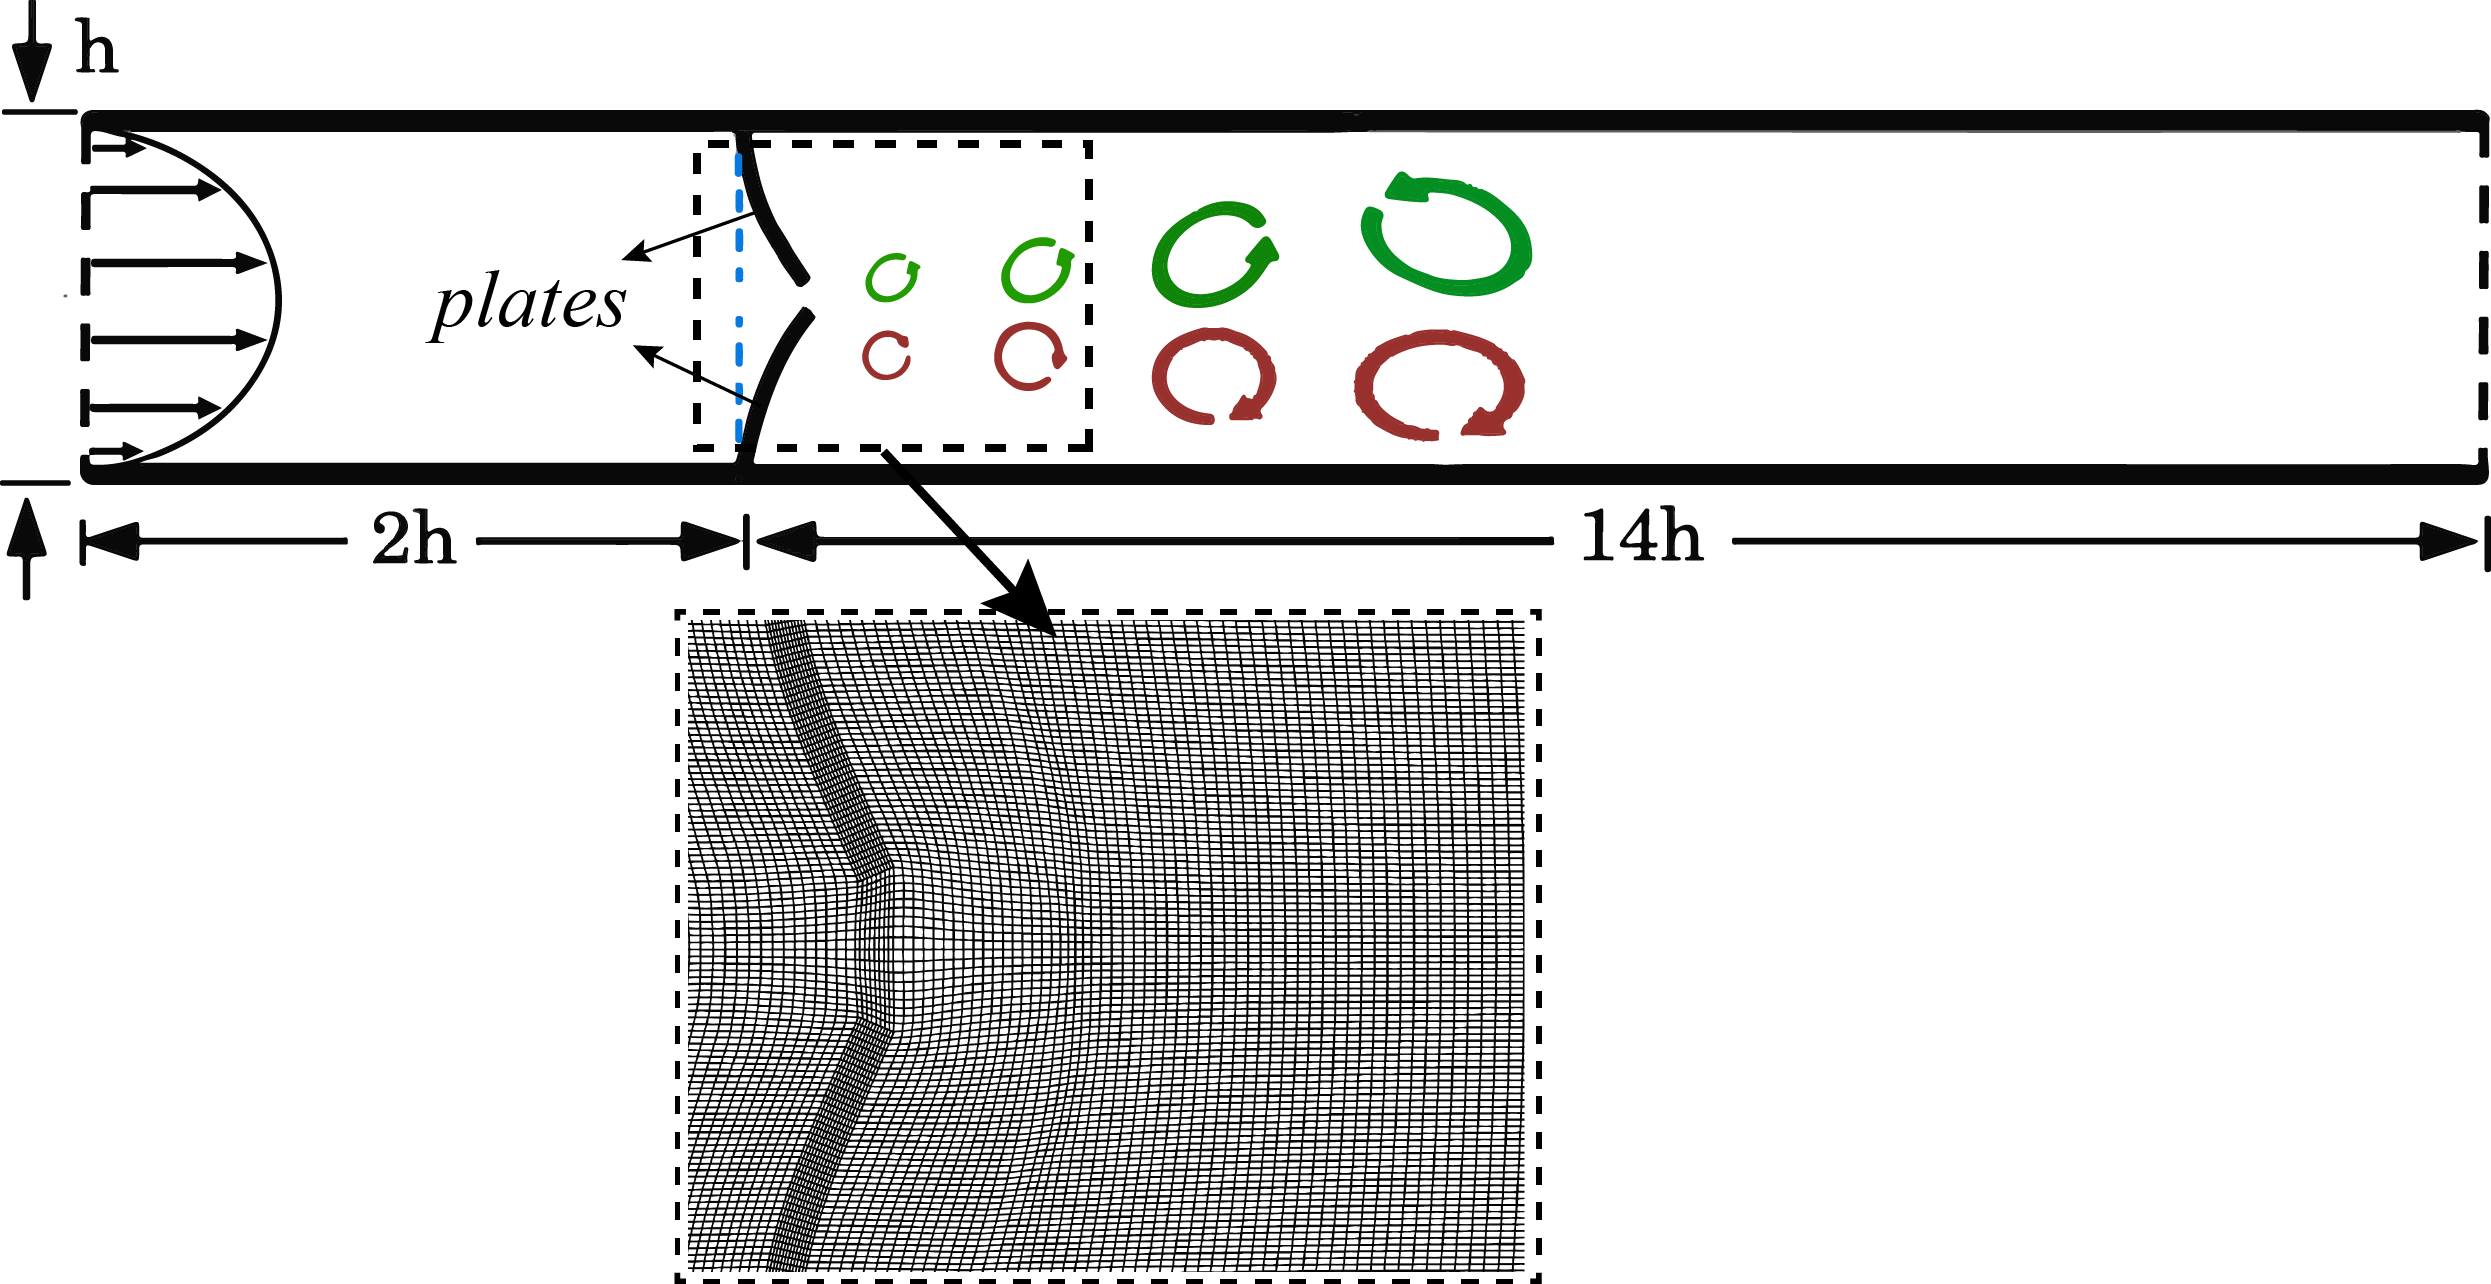
\includegraphics[width=1\linewidth]{Figures/Schematic-01.png} 
			
		\end{minipage} 		
		\caption{Schematic of the fluid flow past wall-mounted flexible plates in a channel. A fully developed flow enters from the inlet (left), passes through the slit between the two oppositely mounted plates, and leaves the channel from the outlet (right). Due to the flexibility of the mounted plates, the slit gap varies under the effect of inlet flow and causes vortical flow structures in the downstream domain. A typical mesh grid used is shown for the near-plate section of the channel featuring dynamic mesh motion.}	
		\label{fig:schematic}
	\end{figure}
	
	
	\section{Methods}\label{sec:maths}
	\subsection{Governing equations and the numerical method}\label{subsec:maths}
	We have performed numerical simulations of the discussed in the schematic problem. The simulations consist of interaction between the plates and the fluid coupled strongly so as to exchange forces in both ways. The finite volume method of numerical simulations is performed without any turbulence models. the plates' motion is a result of the dynamic interaction between incoming flow and the plates' feedback. The governing equations for the flow are the two-dimensional, incompressible, unsteady Navier-Stokes equations which read as
	\begin{eqnarray}
		\nabla\cdot\left[(\mathbf{u}_f-\mathbf{u}_m)\right] &=& 0, \\
		\rho_f\left[{\partial\mathbf{u}_f\over\partial t}+\left[(\mathbf{u}_f-\mathbf{u}_m)\cdot\mathbf{\nabla}\right]\mathbf{u}_f\right] &=& \mathbf{\nabla}\cdot\mathbf{\boldsymbol{\sigma}}_f,
	\end{eqnarray}
	
	where $\mathbf{u}_f=(u_x,u_y)$ is the velocity of the flow, $\mathbf{u_m}$ is the mesh motion velocity, $\rho_f$ is the fluid density, and $\boldsymbol{\sigma}_f$ is the total stress tensor in the fluid. Here, $\mathbf{\nabla}\equiv ({\partial\over\partial x},{\partial\over\partial y})$ is the spatial gradient for two-dimensions (x-y plane) and ${\partial\over\partial t}$ is the partial derivative operator with time.	Divergence of the stress tensor read as $\nabla\cdot\boldsymbol{\sigma}_f=-\mathbf{\nabla}P+\mu_f\mathbf{\nabla}^2\mathbf{u}_f$ for the incompressible and Newtonian fluid, where, $P$ is dynamic pressure, $\mu_f$ is the fluid dynamic viscosity and $\nabla^2$ is laplacian operator. We have considered the strong coupling methodology between the fluid and the plate (structure) so as to accommodate two-way mutual interaction as discussed before. The governing equations for such couplings are formulated by using the Arbitrary Lagrangian Eulerian (ALE) framework, in which the volume change of each grid element between two subsequent time steps is always equal to the volume swept by the mesh, see more details in~\citep{Nguyen2010, Slone2002, CampbellPaterson2011}.  %The plates' motion (or the displacement, $\mathbf{u}_s$), is computed on the Arbitrary Lagrangian framework on which the mesh velocity ($\mathbf{u}_m$) equals the material velocity, i.e., $\mathbf{u}_m\equiv {\partial\mathbf{u}_s\over\partial t}$. The Eulerian mesh (for the fluid) implementation follows $\mathbf{u}_m=0$, and for the Lagrangian mesh, it follows $\mathbf{u}_m=\mathbf{u}_f$.
	The governing equation considered for the flexible plate is given by,	
	\begin{eqnarray}
		\rho_s{\partial^2\mathbf{u}_s\over\partial t^2} &=& \mathbf{\nabla}\cdot\mathbf{\boldsymbol{\sigma}}_s,
	\end{eqnarray}
	where $\rho_s$ is the density of the plate, $\mathbf{u}_s$ is the plates' motion velocity, and $\mathbf{\boldsymbol{\sigma}}_s$ is the Cauchy stress tensor. We have assumed a linear elastic material property for the plate, in which the strain rate is defined as per Lagrangian-Green's tensor, $\boldsymbol{\varepsilon}_s={1\over2}(\mathbf{\nabla}\mathbf{u}_s+\mathbf{\nabla}\mathbf{u}_s^T+\mathbf{\nabla}\mathbf{u}_s^T \cdot \mathbf{\nabla}\mathbf{u}_s)$. The stress and strain tensors are constituted as $\boldsymbol{\sigma}_s=2\mu_s \boldsymbol{\varepsilon}_s+\lambda( \mathbf{\nabla}\cdot\mathbf{u}_s)\mathcal{I}$, where, $\mu_s=\mathcal{E}/[2(1+\kappa)]$ and $\lambda=\kappa \mathcal{E}/[(1+\kappa)(1-2\kappa)]$ are the Lame's constants, $\mathcal{E}$ is the Young's modulus, $\kappa$ is the Poisson's ratio,  and $\mathcal{I}$ is a rank two identity tensor. The superscript $^T$ here represents transpose of a tensor. The information between the fluid stresses and the plates' motion displacement exchange at the interface i.e $\mathbf{u}_m=\mathbf{u}_f$ and $\boldsymbol{\sigma}_s\cdot\mathbf{n}=\boldsymbol{\sigma}_f\cdot\mathbf{n}$,where $\mathbf{n}$ is the normal vector to the wall-fluid interface, see more details in~\citep{CasadeiHalleux1995, Casadei2001}. The suffixes $_f$, $_s$ and $_m$ correspond to fluid, solid and mesh, respectively.
	%We have used the Laplace operator approach to compute the fluid mesh motion by solving $\mathbf{\nabla}\cdot(\gamma\mathbf{\nabla}\mathbf{u}_f)=0$, as mentioned in~\citep{JasakTukovik2006}. Here, $\gamma$ is a variable diffusion coefficient which is inversely proportional to the distance from the moving boundary.
	
	The temporal discretization for the governing equations is done using a second-order Euler-implicit scheme and the spatial discretization of the convection and diffusion terms with Gaussian integration using central differencing method. The Courant number in the simulations are always kept under 0.2 with suitably adjusted time-steps. More details on the process of solution of the governing equations have been discussed in our previous research work\citep{Self2019}.
	We have submitted grid validation results in the same work. Also in figure 2 of \citep{Self2019}, we have computed tip deflection vs time for method validation and compared it with the results mentioned in section 3.1.2 of~\citep{Gluck2001}, which concur with the results our simulations. 
	
	
	
	\subsection{Problem Description and dimensionless parameter}
	
	The flow in a confined channel and ejecting past wall-mounted thin flexible plates are investigated. A schematic of the model as two-dimensional channel geometry of height $h$ and length $14h$ is shown in Fig. \ref{fig:schematic}. Two flexible plates, each of length $l = 0.425h$, are fixed on the opposite walls at a distance of $2h$ from the channel inlet. The thickness of each plate is $b = 0.05h$ and width $w=0.125h$ (into the plane). The inlet flow profile across the channel is set to mimic a fully developed parabolic nature expressed as $u(y)=4u\left(\frac{y}{h}\right)\left(1-\frac{y}{h}\right)$ with zero pressure gradient as boundary conditions. We have considered a steady laminar inlet flow in the channel with maximum inlet Reynolds number as $500$ which is formulated as $Re={\rho_fu_o h}/\mu_f$, where $u_0$ is maximum inlet velocity at mid of the channel height. The outlet boundary conditions are maintained as zero-velocity gradient and fixed (zero) pressure. Additionally, the grid cells along channel length is adjusted in such a way so that the outlet boundary effects are cushioned and do not reflect back into the flow transients . We have applied no-slip conditions on the channel boundary walls and on the fluid-plate interface. The ratio of fluid density to structure density is $\rho_f / \rho_s = 0.02$. The flexibility of the two plates placed on the opposite wall is considered a parameter in the form of the ratio between fluid inertial force to the structural restoring force of the plate, i.e. Cauchy Number, $Ca=\rho_f u_o^2 h^3 b/{\mathcal{E}I} $ where $I=bw^3/12$ is the area moment of inertia of the structure. We have varied $Ca$ in the range of $8\times10^{-9}$ (rigid) to $6\times10^{-2}$. This channel domain ($h\times14h$) is composed of a grid of hexahedral cells as $118$ grid cells along the channel height and $520$ grid cells along its length. The thin plate structures are also computationally discretized into a hexahedral grid as $12$ cells along the thickness and $50$ cells along the plate height for each of the two plates. We have considered time scale factor based on convective motions i.e. $\tau={h/u_o}$ for time parameter. We have simulated our results upto $t/\tau=10$ which we found enough for computing steady state results.
	
	
	\begin{figure}
		\centering
		\begin{minipage}[c]{0.77\linewidth}
			\begin{overpic}[width=0.97\linewidth,height=1.5cm,trim=100 0 600 0, clip]{Figures/Figures/Jet/1S/1S_0100.png}
				\put(-25,20){{\parbox{0.4\linewidth}{$(a)$}}}
				\put(70,20){{\parbox{0.4\linewidth}{$LVP$}}}
			\end{overpic}
			%	\tikz \draw (0,0) ellipse (2cm and 1cm)
			\begin{overpic}[width=0.97\linewidth,height=1.5cm,trim=100 0 600 0, clip]{Figures/Figures/Jet/1S/1S_0500.png}
				\put(-25,20){{\parbox{0.4\linewidth}{$(b)$}}}
			\end{overpic}
			\begin{overpic}[width=0.97\linewidth,height=1.5cm,trim=100 0 600 0, clip]{Figures/Figures/Jet/1S/1S_0950.png}
				\put(-25,20){{\parbox{0.4\linewidth}{$(c)$}}}
				\put(60,27){{\parbox{0.4\linewidth}{$trailing \ shear \ layer$}}}
			\end{overpic}
			\begin{overpic}[width=0.97\linewidth,height=1.5cm,trim=100 0 600 0, clip]{Figures/Figures/Jet/1S/1S_1400.png}
				\put(-25,20){{\parbox{0.4\linewidth}{$(d)$}}}
				\put(160,8){{\parbox{0.4\linewidth}{$detachment$}}}
			\end{overpic}		
			%		\begin{overpic}[width=0.97\linewidth,height=1.5cm,trim=100 0 600 0, clip]{Figures/Figures/Jet/1S/1S_1850.png}
				%			\put(-25,20){{\parbox{0.4\linewidth}{$(e)$}}}
				%		\end{overpic}
		\end{minipage}
		\begin{minipage}[c]{0.03\linewidth}
			\centering
			\begin{overpic}[width=0.75\linewidth,height= 3.5cm]{Figures/Figures/Jet/1S/leg3.png}
				\put(14,52){{\parbox{0.4\linewidth}{\rotatebox{90}{\Large$u_x/u_o$}}}}
				\put(14,95){{\parbox{0.4\linewidth}{\Large$8$}}}
				\put(14,2){{\parbox{0.4\linewidth}{\Large$1$}}}		
			\end{overpic}
		\end{minipage} 
		\caption{Contour of instantaneous stream-wise velocity of the flow through slit between the rigid plates normalised by the inlet flow velocity $u_x/u_0$. Time snapshots are at instances $t/\tau \approx 7,\ 35,\ 70,\ 103 $ for each panel respectively.}
		\label{fig:Ux_contour_1S}
	\end{figure}
	
	
	\begin{figure}
		\begin{minipage}[c]{1\linewidth}	
			\begin{overpic}[width=1\linewidth]{Figures/unconfined/1fixbc_100_400_1400.png}
				\put(-230,335){{\parbox{1\linewidth}{$(a)$}}}
			\end{overpic}
		\end{minipage}
		
		\caption{Evolution of vorticity contours through the narrow slit in an unbounded case at three different time instances.(a) $t/\tau\approx7$, (b) $t/\tau\approx28$, and (c) $t/\tau\approx100$. Sub-figure (b) also presents a sample velocity vector fields.}
		\label{fig:Ux_contour_1S_unbounded}
	\end{figure}
	
	\section{Results and Discussion}\label{sec:Results}
	
	In this study we explore the fluid dynamics in a narrow, slit-like gap formed by two rigid, wall-mounted plates. This analysis is based on the interpretation of the velocity contour, delineated in Figure \ref{fig:Ux_contour_1S}, which provides an illustrative understanding of the flow process through this specific spatial configuration. The investigation focuses on a series of time frames, specifically $t/\tau \approx 7,\ 35,\ 70,\ and \ 103$, whose corresponding flow states are depicted in the sub-panels $(a)-(d)$ of the figure. 
	
	Initially, the fluid enters the slit gap-width $\delta_g$, and experiences acceleration due to the spatial confinement provided by the narrow slit. This leads to a roll-up motion in a direction perpendicular to the flow, giving rise to  a "mushroom"-like structure at the head of the flow. This structure, a distinguishing feature of the flow process in our study, consists of a counter-rotating vortex pair. The resulting formation, henceforth referred to as the 'leading vortex pair' (LVP), follows an evolutionary journey downstream, leaving its mark as the inaugural mass ejection that transpires from the system.
	
	In the context of the formation's interaction with the slit, a trailing shear layer keeps the LVP connected with the slit edges, making its way downstream. This layer grows in congruity with the self-similar growth pattern of the LVP, a phenomenon that is evident from the subsequent panels of Figure \ref{fig:Ux_contour_1S}. However, an important aspect of this system is the boundary conditions imposed by the channel walls, which appear to restrict the growth of the LVP.
	
	To further illuminate this aspect, a comparative analysis is presented, considering a similar fluid dynamic situation but with wider channel openings. This scenario, portrayed in Figure \ref{fig:Ux_contour_1S_unbounded}, can be deemed to replicate an "unbounded" case, where there are minimal restrictions on the flow growth. From the panels in the figure, it is apparent that the mushroom-shaped ejection experiences unimpeded growth, contrasting with the in-channel or "bounded" flow case. Furthermore, in panel $(b)$ of this figure, a representative velocity vector field and vorticity outlines are provided for comparison.
	
	The discussion thus far has concentrated on the flow's early evolution and the formation of the leading vortex pair. However, this leading pair is not invulnerable to destabilization. As the flow moves further downstream, the LVP becomes unstable, as shown in panel $(c)$. To gain a deeper understanding of this phenomenon and the early flow development process, a mathematical model is proposed in the subsequent subsection.
	
	\subsection{Mathematical Model: Formation and Growth of the Leading Vortex Pair}\label{sec:model}
	
	In the given setting, we formulate a mathematical model, encompassing the formation and growth of the initial vortex pair. This vortex pair, resulting from the roll-up of the trailing shear layer attached to the slit, is assumed to draw in all the fluid entering the slit gap. Upon formation, this vortex pair adopts an approximately circular shape and displays a degree of self-similar radial growth. However, as the trailing shear layer elongates over time, an instability develops, which terminates the radial growth of the LVP. This process is depicted schematically in Figure \ref{fig:model}. The model assumes that the fluid enters the slit at a constant velocity, denoted as $u_o$. As the fluid travels over time, it forms a circular blob-like structure near the slit, characterized by a radius $r$.
		\begin{figure}
		\centering
		\begin{minipage}[c]{1\linewidth}	
			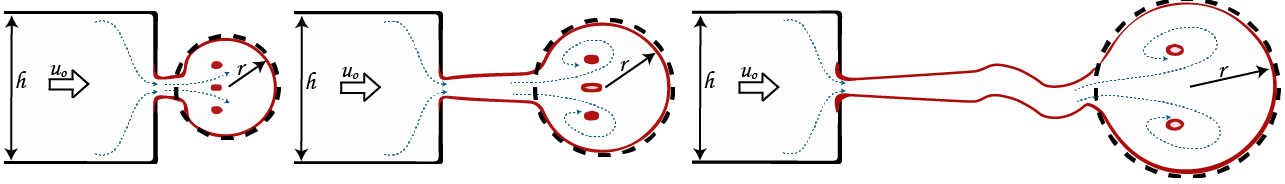
\includegraphics[width=1\linewidth]{Figures/VortexPair/model_100_200_400_3.png}
		\end{minipage}
		
		\caption{(a) Illustration of flow evolution through the narrow slit to an unbounded opening case. The dashed circle in each panel marks an approximation of the starting flow in a circular shape of radius $r$. A slug flow is assumed as inlet with velocity $u_o$ in a channel of width $h$.}
		\label{fig:model}
	\end{figure}
		\begin{figure}[h]
	\centering
	\begin{minipage}[c]{0.58\linewidth}
		\centering
		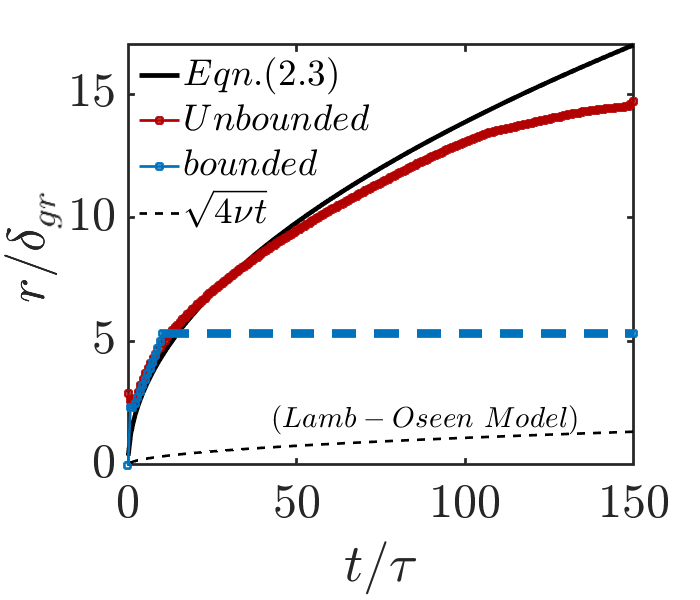
\includegraphics[width=1\linewidth] {Figures/radius_model2.png} 
	\end{minipage}
	\caption{Radius of the rolled-up starting flow evolution for the unbounded and bounded case with proposed growth model (solid black line) with time. A sample growth rate due to viscous diffusion (Lamb-Oseen Model) is shown in black dashed line for comparison.}
	\label{fig:model}
\end{figure}
	A crucial parameter in our model is the discharge coefficient, which is assumed to be 1, implying that the fluid volume discharged through the slit equals the volume of fluid entering the channel. By considering the inlet fluid volume as a column of fluid entering at a velocity $u_o$, the total fluid discharged over time, represented as $Q_{in}$, can be mathematically expressed as:
	
	\begin{equation}
		Q_{in}=\int_{0}^{t}u_o hdt = \int_{0}^{t}u_g \delta_gdt
		\label{eqn:Q_in}
	\end{equation}
	
	This equation essentially encapsulates the conservation of mass principle by equating the volume of fluid entering the system (inlet) with the volume discharged over time.
	
	Within the context of the leading vortex pair, the fluid accumulation in the circular, disk-shaped blob due to the roll-up of the shear layers displays a self-similar growth pattern in terms of its radius, $r(t)$. This observation allows us to represent the volume flow rate stored in the leading vortex pair, $Q_{lvp}$, in the following manner:
	
	\begin{equation}
		\int_{0}^{t}Q_{lvp}dt= \pi r^2(t)
		\label{eqn:Q_lvp}
	\end{equation}
	
	Here, the integral of the volume flow rate over time gives the volume of the fluid collected in the LVP, which is geometrically akin to the volume of a disk of radius $r(t)$.
	
	By making two essential assumptions: no entrainment effects (i.e., no additional fluid is drawn into the flow beyond what enters the slit) and a negligible trailing layer volume, we can infer that the volume flow rate entering the slit equals the volume flow rate stored in the LVP, i.e., $Q_{in}$ $=$ $Q_{lvp}$. Consequently, this allows us to derive the growth of the leading vortex pair, linking it with the equations \ref{eqn:Q_in} and \ref{eqn:Q_lvp}, which results in the following relationship:
	
	\begin{equation}
		r(t) = \sqrt{\frac{u_o h}{\pi}t}
		\label{eqn:r_lvp}
	\end{equation}
	
	This mathematical expression encapsulates the crux of our model, capturing the radius of the leading vortex pair as a function of time, $r(t)$, in terms of the inlet velocity $u_o$, channel height $h$, and time $t$. This model offers a analytical framework to comprehend the behavior of the leading vortex pair during the early stages of flow through a narrow slit. 
	
	To illustrate the derived relation between the radius growth with respect to time, figure \ref{fig:model} show the curve in black line for \ref{eqn:r_lvp}. We present the growth of the leading head for both bounded and unbounded starting flow through the slit as discussed. In case of the unbounded flow evolution, the radius growth trend matches with the proposed relation unto an initial time period, but at later times the growth trend shows a deviation. This is because of the no-entrainment and negligible trailing flow assumptions for the model proposition as the assumed conditions begin to fail as the flow extends longer into the downstream. For the bounded in-channel flow evolution, the initial growth can be observed to follow the proposed relation. But due to the wall confinements in either directions this growth gets hindered and the leading patch no longer remains circular disc instead extends laterally under the effect of wall boundaries. The growth curve for the bounded case is shown in the same figure as blue line. The thick dashed blue line marks the channel width in the plot which indicate the growth limits. We have also shown a typical viscous diffusion rate of a Lamb-Oseen vortex with constant circulation  as a standard reference for comparison. This diffusion based growth rate is much lower than in the present case of attached shear layer based influx growth.
	
	
	
	\begin{figure}
		\centering
		\begin{minipage}[c]{0.77\linewidth}
			\vspace{0.7cm}
			\begin{overpic}[width=0.97\linewidth,height=1.5cm,trim=10 120 400 120, clip]{Figures/Figures/Jet/1S/1S_vort_100.png}
				\put(-25,20){{\parbox{0.4\linewidth}{$(a)$}}}
			\end{overpic}
			\begin{overpic}[width=0.97\linewidth,height=1.5cm,trim=10 120 400 120, clip]{Figures/Figures/Jet/1S/1S_vort_500.png}
				\put(-25,20){{\parbox{0.4\linewidth}{$(b)$}}}
				\put(160,24){{\parbox{0.4\linewidth}{$LVP$}}}
			\end{overpic}
			\begin{overpic}[width=0.97\linewidth,height=1.5cm,trim=10 120 400 120, clip]{Figures/Figures/Jet/1S/1S_vort_1000.png}
				\put(-25,20){{\parbox{0.4\linewidth}{$(c)$}}}
			\end{overpic}
			\begin{overpic}[width=0.97\linewidth,height=1.5cm,trim=10 120 400 120, clip]{Figures/Figures/Jet/1S/1S_vort_1400.png}
				\put(-25,20){{\parbox{0.4\linewidth}{$(d)$}}}
				\put(80,29){{\parbox{0.4\linewidth}{$trailing \ shear \ layer$}}}
			\end{overpic}		
			\begin{overpic}[width=0.97\linewidth,height=1.5cm,trim=10 120 400 120, clip]{Figures/Figures/Jet/1S/1S_vort_1600.png}
				\put(-25,20){{\parbox{0.4\linewidth}{$(e)$}}}
			\end{overpic}
		\end{minipage}
		\begin{minipage}[c]{0.04\linewidth}
			\begin{overpic}[width=1\linewidth,height= 4.5cm]{Figures/Figures/Jet/leg_vort.png}
				\put(15,62){{\parbox{0.4\linewidth}{\rotatebox{90}{\Large$\Omega$}}}}
				\put(15,105){{\parbox{0.4\linewidth}{\Large$5$}}}
				\put(10,20){{\parbox{0.4\linewidth}{\Large$-5$}}}		
			\end{overpic}
			\vspace{0.2cm}
		\end{minipage}
		\caption{Contour of instantaneous vorticity contour of the flow through slit between the rigid plates. Time snapshots are at instances $t/\tau \approx 7,\ 36,\ 73,\ 103, \ and \ 117 $ for each panel respectively.}
		\label{fig:Vort_contour_1S}
	\end{figure}
	\begin{figure}
		\centering
		\begin{minipage}[c]{0.46\linewidth}
			\centering
			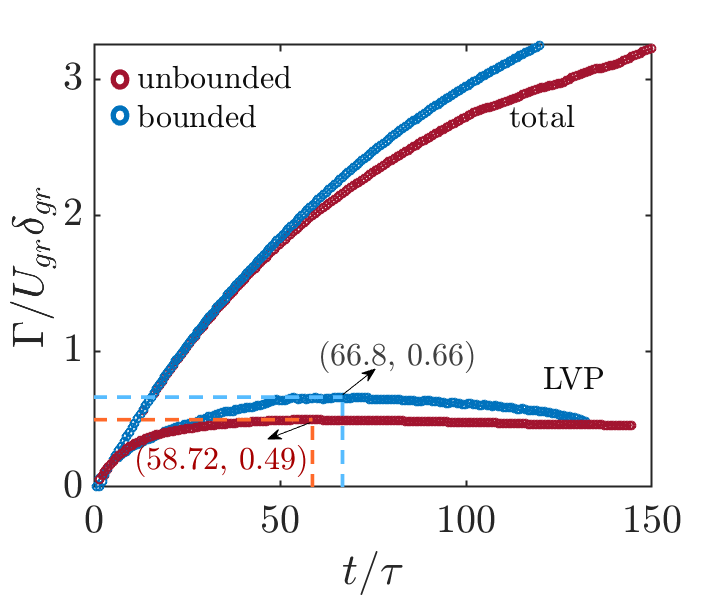
\includegraphics[width=1\linewidth] {Figures/Circ_S1.png} 
		\end{minipage}
		\begin{minipage}[c]{0.495\linewidth}
		\centering
		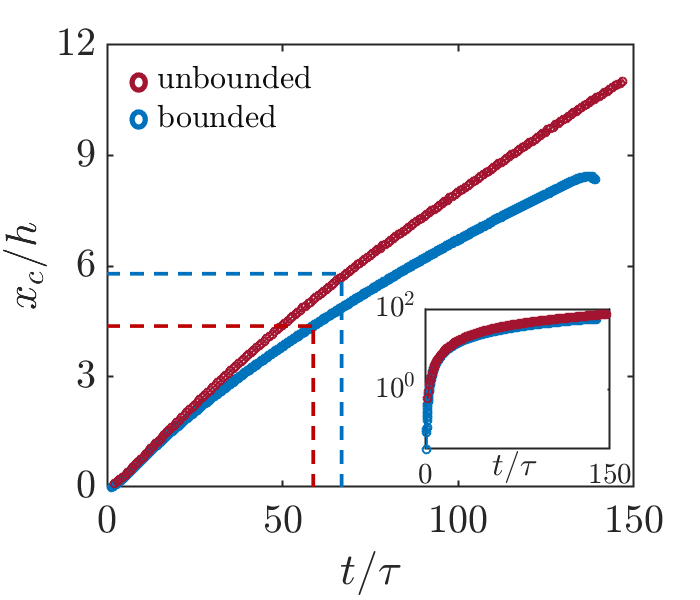
\includegraphics[width=1\linewidth] {Figures/velocity.png} 
	\end{minipage}
		\caption{(a) Time evolution of the vortex circulation, normalized by the velocity and width at the slit ($\Gamma$/$u_g\delta_g$) for net ejected flow and also for leading vortex pair (LVP). The dashed lines mark the maxima of the accumulated circulation within the LVP and hints its detachment.(b) Position trace of the leading vortex pair (LVP) for unbounded and bounded case. The subplot inside shows semi-log plot to show corresponding change in the position steepness.}
		\label{fig:Circ_S1_vs_T}
	\end{figure}


	To show the aforementioned vortex pair roll-up, we present the vorticity contour for the flow through slit from rigid plates in figure \ref{fig:Vort_contour_1S} at different time instants. Time snapshots are at instances $t/\tau \approx 7,\ 36,\ 73,\ 103, \ and \ 117 $ for each panel respectively. In the vorticity contour, red colour indicates counter-clockwise rotation, and blue colour indicates clockwise rotation of the flow (contour is identified at  $\approx  5\%$ of maximum vorticity). The figure shows the roll-up near the slit gap and its streamwise extension into the downstream over time. After a certain length of extension, the shear layer instigates Kelvin-Helmholtz instability and the LVP begins to dissociate from its tail (see figure \ref{fig:Vort_contour_1S} (e)).  Also the effect of wall confinement can be noticed as some vorticity is generated on the either walls near the LVP. Due to this confinement effect, the fluid shear gets increased and generates larger vorticity. In the figure \ref{fig:Circ_S1_vs_T}(a), total circulation released off the rigid plates' edges is shown for both bounded and unbounded cases. We have calculated this circulation by considering positive half of the vorticity in the complete downstream domain past the slit gap. Also the circulation is normalised by slit gap-width and mean velocity through the slit-gap to result into a non-dimensional scaling factor ($\Gamma/u_g\delta_g$). In the figure, the curves show that the bounded case attains larger circulation over time when compared to the unbounded case. This is due to the effect of confined walls which induce additional velocity gradients into the domain than those in the unbounded case. The same figure also shows the circulation entrapped in the flow head or the leading vortex (LVP). We can observe the similar results as in the case of total circulation as the leading vortex pair grows and gets closer to the walls thereby generates more shear against the wall boundaries. However, this process of accumulating vorticity from the inlet source is not indefinite and the LVP attains a maximum circulation value. We have shown the point as dashed line with coordinates in the same figure which marks the startup time of the LVP. The start-up time for bounded and unbounded case is identified as $\approx$ $68$ and $\approx \ 59$ respectively. Thus, it can be concluded that the bounded in-channel setting causes a delay in start-up time of the vortex pairs and thereby pull more vorticity into them.
		\begin{figure}
		\centering
		\begin{minipage}[c]{0.495\linewidth}
			\centering
			\begin{overpic}[width=1\linewidth]{Figures/Figures/time-space_S1_fixbc.png}
				\put(135,40){{\parbox{0.4\linewidth}{\rotatebox{0}{$unbounded$}}}}
				\put(70,65){{\parbox{0.1\linewidth}{\rotatebox{30}{$LVP$}}}}	
			\end{overpic}
		\end{minipage}
		\begin{minipage}[c]{0.495\linewidth}
			\centering
			\begin{overpic}[width=1\linewidth]{Figures/Figures/time-space_S1.png}
				\put(145,40){{\parbox{0.3\linewidth}{\rotatebox{0}{$bounded$}}}}
				\put(68,68){{\parbox{0.1\linewidth}{\rotatebox{40}{$LVP$}}}}
				%		\put(15,105){{\parbox{0.4\linewidth}{\Large$2.5$}}}
				%		\put(10,20){{\parbox{0.4\linewidth}{\Large$-2.5$}}}		
			\end{overpic}
		\end{minipage}
		\caption{Space-time map of the vertically integrated vorticity for bounded case. The continuous line is the automatically detected centre of the separated vortex, the dashed lines are the estimated vortex boundaries.}
		\label{fig:time_space}
	\end{figure}
	The LVP at this instant cuts off from the attached trailing layer due to the aforementioned K-H instability. The dissociated LVP begins to decay and past this start-up time and the vortex core deviates from its rectilinear trajectory at later time instant. The counter rotating vortex pairs are self-propagating and hence they even travel even after its dissociation but at a slower rate.
	Figure \ref{fig:Circ_S1_vs_T}(b) show the position track of the leading vortex core normalised over  $(xc)$ over time. We can observe in the figure that the traverse rate of vortex core is slower than that in the unbounded domain case. As explained before, the boundary walls induce an additional shear onto the LVP and hence resists the rate of its downstream propagation. Additionally, the vortex pair also show gradual change in the rate of propagation based on their startup phenomena. The dashed line in the same figure marks the start-up time. As discussed previously, the induction of vorticity in the vortex pair cuts-off at the start-up time and thus no longer receives any direct inertial force from the inlet. Still, under the effect of advection the and due to the self-propagating nature of the dipole, the LVP moves at a slightly lower rate. The sub-panel in the figure show semi-log plot for the same with vortex core downstream position as logarithmic scale. We have only shown the LVP until it is distinctly identifiable but as the shear layer instability kicks-in at later times, the rotating and counter-rotating part of the LVP arrange in alternating fashion in the downstream. Figure \ref{fig:time_space} show the space-time map of the vertically integrated vorticity for unbounded and bounded case in left and right panel respectively. The vorticity pattern in this figure imprints the trail of LVP  over time in the figure. After the LVP dissociates from the trailing shear layer, subsequent vortices form behind it imprint of which can be seen in the space-time map as fringe patterns which corresponds to the arrangement of dissociated vortices in alternating fashion. An early lateral spread of these released vortices is a noticeable difference in the case of unbounded case with that of bounded case.
	\begin{figure}
	\begin{center}
		\begin{minipage}[c]{0.49\linewidth}	
			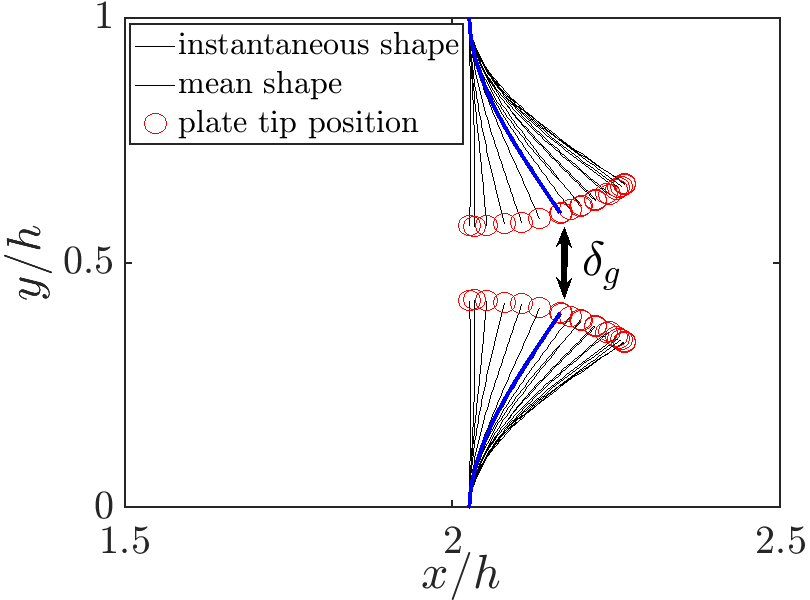
\includegraphics[width=1\linewidth]{Figures/def_shape2.png}\\
			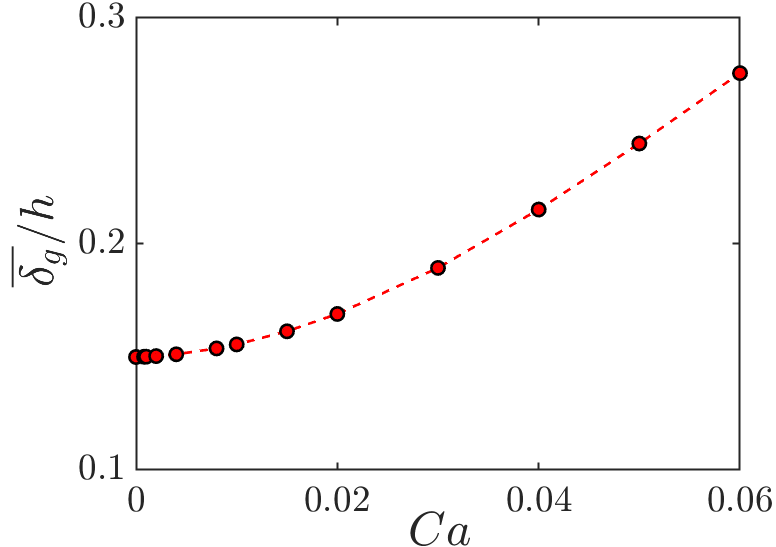
\includegraphics[width=1\linewidth]{Figures/gap_signal/gap_steady2.png}
		\end{minipage}
		\begin{minipage}[c]{0.49\linewidth}	
			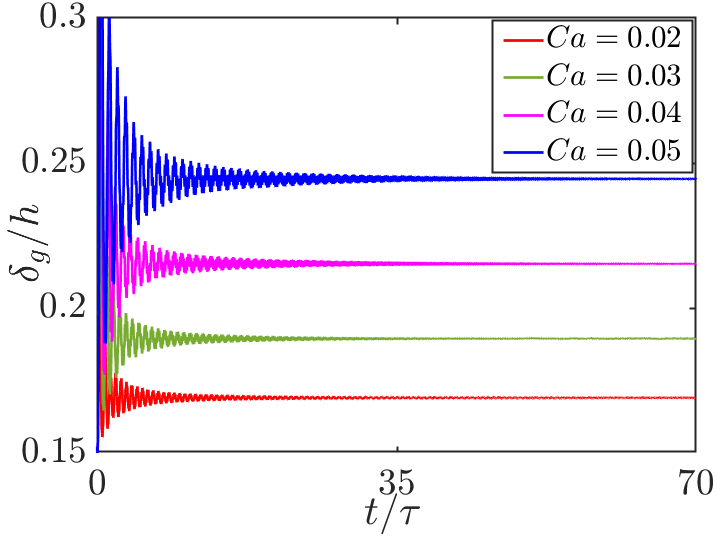
\includegraphics[width=1\linewidth]{Figures/gap_signal/gap_sig_3_4p1_5_5p1S-2.png}
			\begin{overpic}[width=0.95\linewidth]{Figures/drag/Cd_parabolic_S.png}
				\put(-230,335){{\parbox{1\linewidth}{$(a)$}}}	
				\put(-0,335){{\parbox{1\linewidth}{$(b)$}}}
				\put(-230,165){{\parbox{1\linewidth}{$(c)$}}}	
				\put(0,165){{\parbox{1\linewidth}{$(d)$}}}
			\end{overpic}
		\end{minipage}
	\end{center}
	\vspace{-10px}
	\caption{(a) Stroboscopic representation of the flexible plate deflection for a sample case. The slit gap ($\delta_g$) between the two plates increases as the plate deflects more under the flow. The thick blue line marks the mean position of the plate. (b) Time history of slit gap width normalized by the channel height ($\delta_g/h$) for plates with varying flexibility (i) $Ca=0.008$ (ii) $Ca=0.02$ (iii) $Ca=0.04$. (c) Trend of the mean slit gap width over the oscillatory steady state for different $Ca$.
		(a) Coefficient of drag ($Cd$) offered by the plates normalized by the drag offered by rigid plates.}
	\label{fig:del_g_vs_Ca_steady}
\end{figure}

	\begin{figure}
	\centering
	\begin{minipage}[c]{0.77\linewidth}
		\vspace{0.7cm}
		\begin{overpic}[width=0.97\linewidth,height=1.5cm,trim=10 120 600 120, clip]{Figures/Figures/Jet/1S/4p1S_0050.png}
			\put(-25,20){{\parbox{0.4\linewidth}{$(a)$}}}
		\end{overpic}
		\begin{overpic}[width=0.97\linewidth,height=1.5cm,trim=10 120 600 120, clip]{Figures/Figures/Jet/1S/4p1S_0100.png}
			\put(-25,20){{\parbox{0.4\linewidth}{$(b)$}}}
			%				\put(160,24){{\parbox{0.4\linewidth}{$LVP$}}}
		\end{overpic}
		\begin{overpic}[width=0.97\linewidth,height=1.5cm,trim=10 120 600 120, clip]{Figures/Figures/Jet/1S/4p1S_0150.png}
			\put(-25,20){{\parbox{0.4\linewidth}{$(c)$}}}
		\end{overpic}
		\begin{overpic}[width=0.97\linewidth,height=1.5cm,trim=10 120 600 120, clip]{Figures/Figures/Jet/1S/4p1S_0300.png}
			\put(-25,20){{\parbox{0.4\linewidth}{$(d)$}}}
			\put(360,5){{\parbox{0.4\linewidth}{$Ca=0.03$}}}
		\end{overpic}		
	\end{minipage}
	\begin{minipage}[c]{0.04\linewidth}
		\begin{overpic}[width=1\linewidth,height= 4.5cm]{Figures/Figures/Jet/leg_vort.png}
			\put(15,62){{\parbox{0.4\linewidth}{\rotatebox{90}{\Large$\Omega$}}}}
			\put(15,105){{\parbox{0.4\linewidth}{\Large$5$}}}
			\put(10,20){{\parbox{0.4\linewidth}{\Large$-5$}}}		
		\end{overpic}
		\vspace{0.2cm}
	\end{minipage}
	\caption{Contour of instantaneous vorticity contour of the flow through slit between the flexible plates with $Ca=0.03$. Time snapshots are at instances $t/\tau \approx 3,\ 7,\ 11,\ and \ 22 $ for each panel respectively.}
	\label{fig:Vort_contour_4S}
\end{figure}
	\subsection{Effect of flexible plates on vortex generation}
	As per our quest to cause early dissociation or to induce a pinch-off phenomena in the vortex pair cases, we investigate the role of flexible plates mounted on opposite walls which form the slit gap (as shown in figure \ref{fig:schematic}). Flexible bodies subjected to an incoming flow gradually deform if fluid inertia begins to outweigh bending stiffness \citep{Shelley2011}. As a result, the structure reshapes to get streamlined, the projected area perpendicular to the flow lowers, and the overall drag force reduces. This reconfiguration of flexible structures under a parabolic inlet flow profile can be seen in our case in figure \ref{fig:del_g_vs_Ca_steady} (a). The stroboscopic visualization shows the initial transients of the plates' shape reconfiguration. The figure corresponds to the case with $Ca = 0.04$ under the incoming steady flow at $Re=500$. The plates bend along their length with a maximum deflection at the tip, i.e. the free end. The tip is represented as the red circles in the figure over the thin black temporal sequence of plate positions. Initially, in the transient state, the plates undergo maximum deformation along the incoming flow, which amounts to nearly half the plate length. However, the plate achieves a mean position in a steady-state inlet and oscillates about it. This mean position is represented by the thick blue shape of the plates in the figure. The two oppositely mounted plates resemble a two-dimensional narrow slit for the flow inlet. However, for the flexible plate model, the system can be assumed as a slit of time-varying opening size (gap). This variation depends on the flow inlet frequency and the other intricate dynamics, which we shall analyze in the later sections. The mean gap-width, $\delta_g$, i.e. the gap between the tips of the two plates in mean position (thick blue line in figure \ref{fig:del_g_vs_Ca_steady})(a), varies as per the inlet fluid forces in comparison to the structural forces, which act over the plates as cantilever loading, as discussed earlier. The detailed analysis of the structural behaviour of such plates under uniform flow conditions is previously studied in our work \citep{Self2019}. We compared the wall-mounted plates with a typical spring-mass-damper model and approximated the vibration analysis, including damping the plate oscillation from transient to steady-state.
	
	\begin{figure}[h]
		\centering
		\begin{minipage}[c]{0.65\linewidth}
			\begin{overpic}[width=1\linewidth, trim=10 119 900 119,clip]{Figures/Figures/Jet/vort/1S_0300.png}
				\put(-50,20){{\parbox{1\linewidth}{$rigid$}}}
			\end{overpic}
			\begin{overpic}[width=1\linewidth, trim=10 119 900 119,clip]{Figures/Figures/Jet/vort/2p3S_0300.png}
				\put(-58,20){{\parbox{1\linewidth}{$Ca=0.001$}}}
			\end{overpic}
			\begin{overpic}[width=1\linewidth, trim=10 119 900 119,clip]{Figures/Figures/Jet/vort/3p1S_0300.png}
				\put(-58,20){{\parbox{1\linewidth}{$Ca=0.015$}}}
			\end{overpic}
			\begin{overpic}[width=1\linewidth, trim=10 119 900 119,clip]{Figures/Figures/Jet/vort/4S_0300.png}
				\put(-58,20){{\parbox{1\linewidth}{$Ca=0.02$}}}
			\end{overpic}
			\begin{overpic}[width=1\linewidth, trim=10 119 900 119,clip]{Figures/Figures/Jet/vort/4p1S_0300.png}
				\put(-58,20){{\parbox{1\linewidth}{$Ca=0.03$}}}	
			\end{overpic}
			\begin{overpic}[width=1\linewidth, trim=10 119 900 119,clip]{Figures/Figures/Jet/vort/5S_0250.png}	
				\put(-58,20){{\parbox{1\linewidth}{$Ca=0.04$}}}		
			\end{overpic}
			\begin{overpic}[width=1\linewidth, trim=10 119 900 119,clip]{Figures/Figures/Jet/vort/6S_0300.png}	
				\put(-58,20){{\parbox{1\linewidth}{$Ca=0.06$}}}		
			\end{overpic}
		\end{minipage}
		\caption{Instantaneous vortex contour for steady inflow past the slit for cases with rigid plates and flexible plate cases with $Ca=0.0008$ to $Ca=0.06$. (top to bottom). See Animation 1 in supplementary attachment.}
		\label{fig:Vort_Ca}
	\end{figure}

	In figure \ref{fig:del_g_vs_Ca_steady}(b), the time-signal variation for the slit opening ($\delta_g$), normalized over the channel height ($h$) is shown for cases of plates' flexibility ($Ca$) under steady flow conditions. Interestingly, all three cases exhibit flutter instability of the plates' tip even in steady flow inlet conditions. These time signals, however, achieve an oscillatory steady-state condition at later times. The mean of the oscillatory steady state of the slit opening ($\overline{\delta_g}$) is scaled with the increasing plates' flexibility, i.e. $Ca=0.0008$ to $Ca=0.06$, in fig. \ref{fig:del_g_vs_Ca_steady}(c). The figure shows a non-linear increase in slit-width and plates' flexibility ($Ca$). The cases with different plates' flexibility can be assumed to be cases of different orifice sizes.
	
	\begin{figure}[h]
		\centering
		\begin{minipage}{0.65\linewidth}
			\begin{overpic}[width=1\linewidth]{Figures/velpro/1S_parabolic_velpro.png}
				\put(-20,0){{\parbox{0.4\linewidth}{$(a)$}}}
			\end{overpic}
			\begin{overpic}[width=1\linewidth]{Figures/velpro/1S_parabolic_umean.png}
			\end{overpic}
			\begin{overpic}[width=1\linewidth]{Figures/velpro/4S_parabolic_velpro.png}
				\put(-20,0){{\parbox{0.4\linewidth}{$(b)$}}}
			\end{overpic}
			\begin{overpic}[width=1\linewidth]{Figures/velpro/4S_parabolic_umean.png}
			\end{overpic}
			\begin{overpic}[width=1\linewidth]{Figures/velpro/6S_parabolic_velpro.png}
				\put(-20,0){{\parbox{0.4\linewidth}{$(c)$}}}
				%	\put(30,-0){{\parbox{0.4\linewidth}{$x/h$}}}
			\end{overpic}
			\begin{overpic}[width=1\linewidth]{Figures/velpro/6S_parabolic_umean.png}
			\end{overpic}
			\begin{overpic}[width=1\linewidth]{Figures/midline/S_midline_parabolic.png}
				\put(155,-10){{\parbox{1\linewidth}{$x/h$}}}
				\put(-20,22){{\parbox{0.4\linewidth}{$(d)$}}}
			\end{overpic}
		\end{minipage}
		\begin{minipage}{0.07\linewidth}
			\begin{overpic}[width=0.7 \linewidth]{Figures/velpro/legend.png}
			\end{overpic}
		\end{minipage}
		\vspace{0.1cm}
		\caption{Time-averaged velocity profiles across the channel at
			nine streamwise locations and time-averaged flow field for plates with varying flexibility cases for (a)rigid (b)$Ca=0.02$, and (c) $Ca=0.06$. (d) Time-averaged centerline Reynolds number ($Re_c$) along the channel’s length normalized by inlet Reynolds number ($Re_\infty$). To guide the eye, dashed horizontal line show the inlet flow $Re_\infty$.}
		\label{fig:velpro_mean}
	\end{figure}
	
		\begin{figure}
		\centering
		\begin{minipage}[c]{0.49 \linewidth}
			\centering
			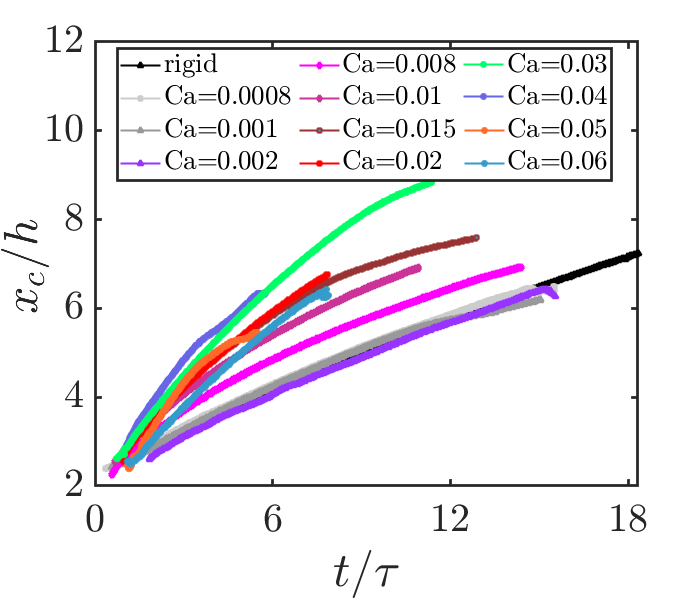
\includegraphics[width=1\linewidth] {Figures/vortProp/vortprop_S_parabolic.png} 
		\end{minipage}
		\begin{minipage}[c]{0.49\linewidth}
			\centering
			%	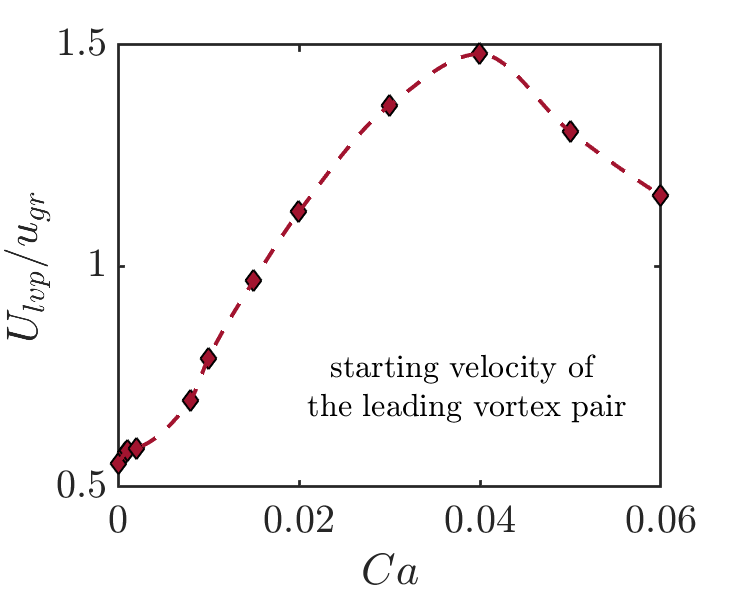
\includegraphics[width=0.985\linewidth] {Figures/vortProp/S_slope.png} 
			\begin{overpic}[width=1\linewidth] {Figures/vortProp/S_slope.png} 
				\put(-240,195){{\parbox{1\linewidth}{$(a)$}}}	
				\put(-5,195){{\parbox{1\linewidth}{$(b)$}}}	
			\end{overpic}
		\end{minipage}
		\caption{Position track of the ejected leading vortex pair over time for the range of $Ca$. (b) Corresponding slope (or starting velocity) for different $Ca$ cases. Maxima of the velocity of the vortex pair at $Ca=0.03$ can be observed.}
		\label{fig:vortPnC}
	\end{figure}
	
	Due to the reconfiguration of the plates under the fluid inertia, a variation in the drag offered by the plates is expected for different $Ca$ cases. In figure \ref{fig:del_g_vs_Ca_steady}(a), the drag co-efficient ($C_d=F_d/0.5\rho_f u_o^2$, where $F_d$ is offered drag force) signal is shown at the steady state reconfigured duration of the simulation. We can observe in the time signals, the transition from no deflection to periodic fluttering as the plates' flexibility is increased. On comparing the mean drag offered by the flexible plates with respect to the rigid plate case, we find an increase in the mean drag until the plates heavily flutter with maximum drag at nearly $Ca=0.01$, shown in \ref{fig:del_g_vs_Ca_steady}(b). This is due to the standing fluid behind the plates which empowers the plates to resist the incoming fluid inertia. Past the fluttering mode i.e. at $Ca>0.01$, the fluid behind the plates gets slightly agitated and gets in even more motion so as to get compliant and lesser resistive. Hence the mean drag is observed to reduce with the increasing plates' flexibility.
	
		\begin{figure}
		\centering
		\begin{minipage}[c]{0.24\linewidth}
			\centering
			%	(a)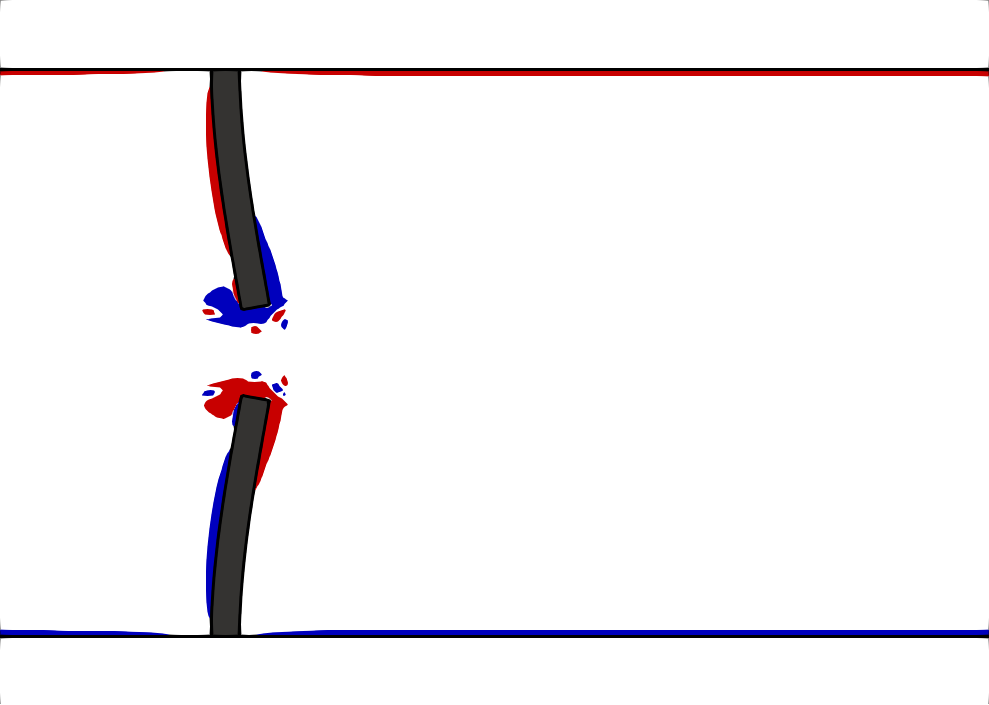
\includegraphics[width=0.7\linewidth]{Figures/5C_selected/5C0006.png}
			\begin{overpic}[width=1\linewidth]{Figures/VortexEvol/1S/1S0015.png}
				\put(0,80){{\parbox{0.4\linewidth}{$(a)$}}}
				\put(-15,37){{\parbox{0.4\linewidth}{$rigid$}}}
			\end{overpic}
			\begin{overpic}[width=1\linewidth]{Figures/VortexEvol/4S/4S0015.png}
				\put(0,60){{\parbox{0.4\linewidth}{$(e)$}}}
				\put(-20,37){{\parbox{1\linewidth}{$Ca=0.02$}}}
			\end{overpic}
			\\$t/\tau=1$
		\end{minipage}
		\begin{minipage}[c]{0.24\linewidth}
			\centering
			%	(a)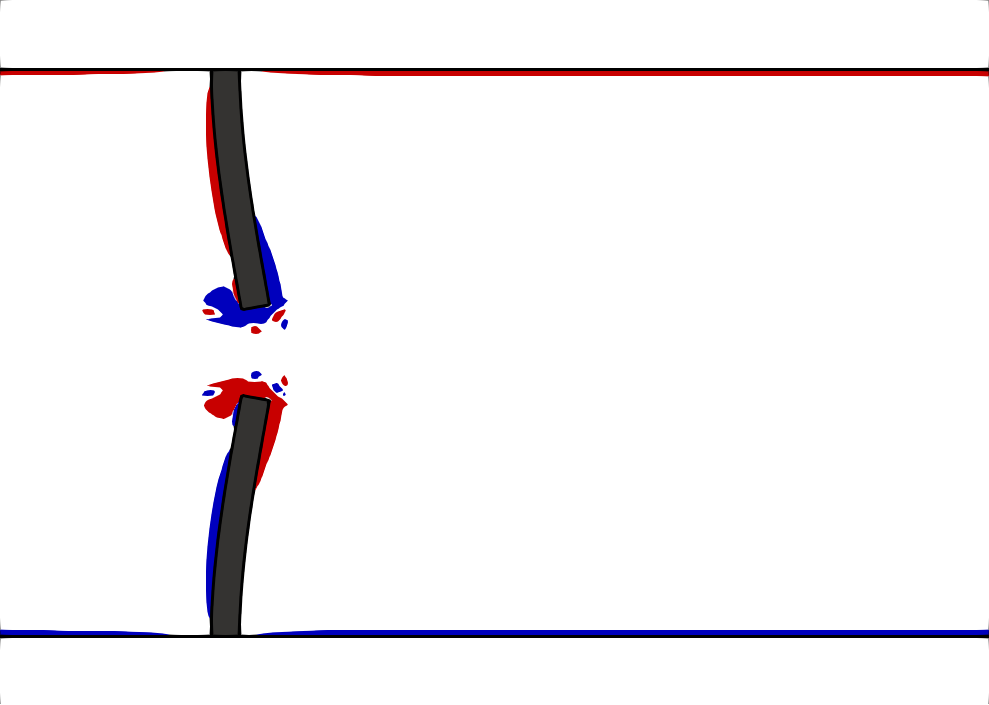
\includegraphics[width=0.7\linewidth]{Figures/5C_selected/5C0006.png}
			\begin{overpic}[width=1\linewidth]{Figures/VortexEvol/1S/1S0025.png}
				\put(0,80){{\parbox{0.4\linewidth}{$(b)$}}}
				%		\put(-75,30){{\parbox{0.4\linewidth}{$t/\tau=0.15$}}}
			\end{overpic}
			\begin{overpic}[width=1\linewidth]{Figures/VortexEvol/4S/4S0025.png}
				\put(0,60){{\parbox{0.4\linewidth}{$(f)$}}}
				%			\put(-75,30){{\parbox{0.4\linewidth}{$t/\tau=0.25$}}}
			\end{overpic}
			\\$t/\tau=1.85$
		\end{minipage}
		\begin{minipage}[c]{0.24\linewidth}
			\centering
			%	(a)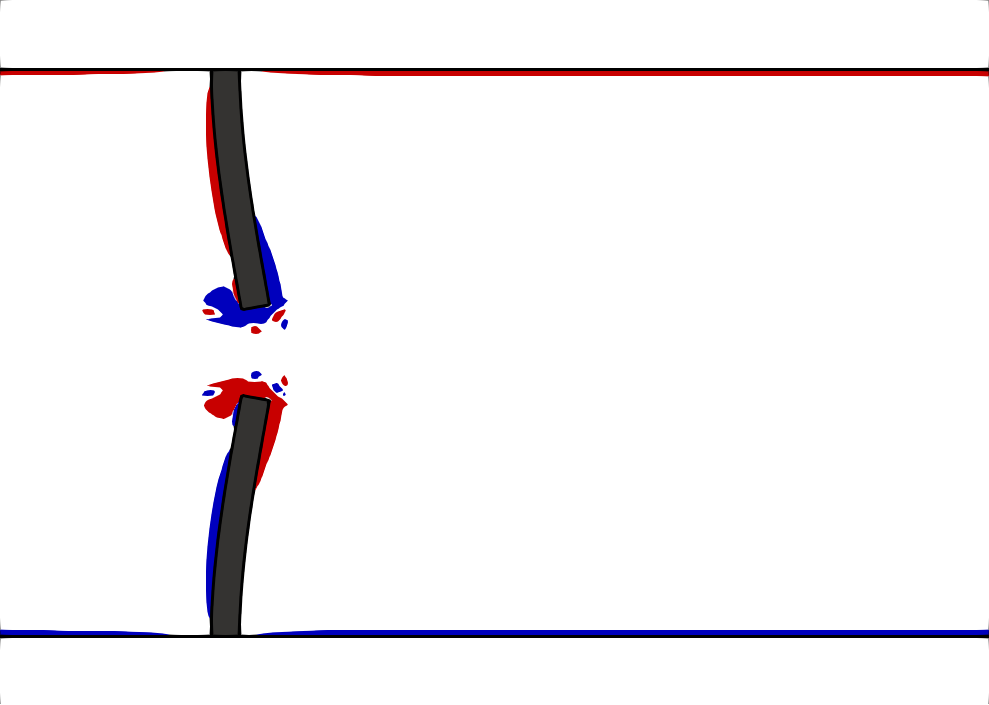
\includegraphics[width=0.7\linewidth]{Figures/5C_selected/5C0006.png}
			\begin{overpic}[width=1\linewidth]{Figures/VortexEvol/1S/1S0045.png}
				\put(0,80){{\parbox{0.4\linewidth}{$(c)$}}}
				%		\put(-75,30){{\parbox{0.4\linewidth}{$t/\tau=0.15$}}}
			\end{overpic}
			\begin{overpic}[width=1\linewidth]{Figures/VortexEvol/4S/4S0045.png}
				\put(0,60){{\parbox{0.4\linewidth}{$(g)$}}}
				%		\put(-75,30){{\parbox{0.4\linewidth}{$t/\tau=0.25$}}}
			\end{overpic}
			\\$t/\tau=3.30$
		\end{minipage}
		\begin{minipage}[c]{0.24\linewidth}
			\centering
			%	(a)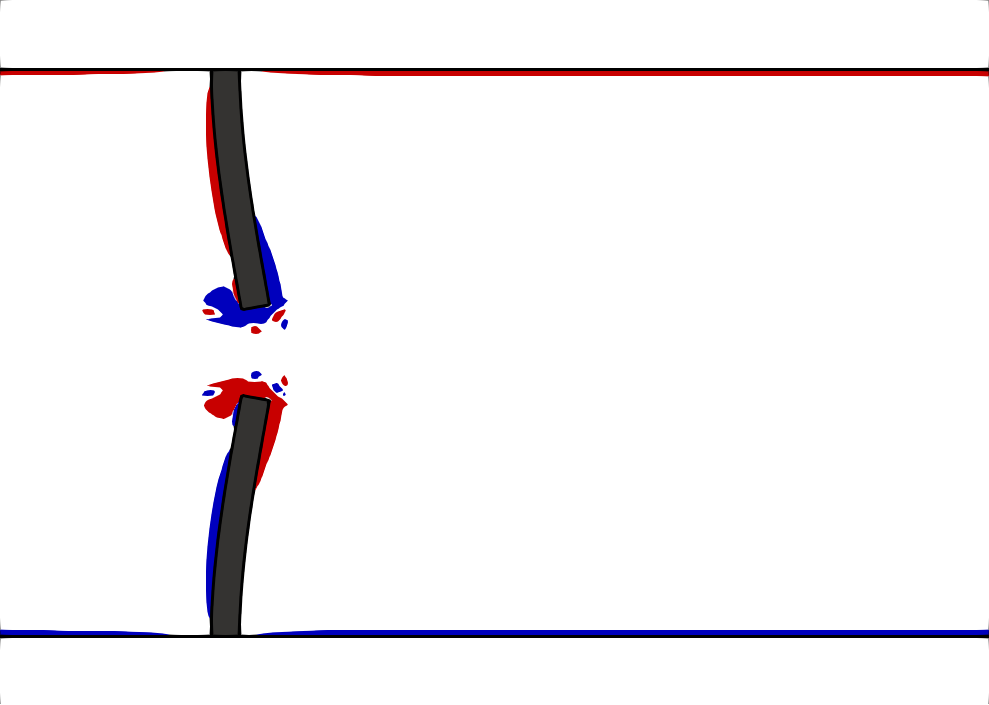
\includegraphics[width=0.7\linewidth]{Figures/5C_selected/5C0006.png}
			\begin{overpic}[width=1\linewidth]{Figures/VortexEvol/1S/1S0065.png}
				\put(0,80){{\parbox{0.4\linewidth}{$(d)$}}}
				%		\put(-75,30){{\parbox{0.4\linewidth}{$t/\tau=0.15$}}}
			\end{overpic}
			\begin{overpic}[width=1\linewidth]{Figures/VortexEvol/4S/4S0065.png}
				\put(0,60){{\parbox{0.4\linewidth}{$(h)$}}}
				%		\put(-75,30){{\parbox{0.4\linewidth}{$t/\tau=0.25$}}}
			\end{overpic}
			\\$t/\tau=4.75$
		\end{minipage}
		\caption{Comparison of starting vortex ejection rigid and flexible plate case. (a) Time sequence of vorticity contours for (a-d) rigid plate case and (e-h) flexible plate case, $Ca=0.02$. The blue and red colour shows clockwise and counter-clockwise vortices respectively}
		\label{fig:vort_evo_1S_4S}
	\end{figure}
	
	In case when flexible plates are used instead of rigid plates to form a narrow slit, the flow evolution can be observed to be significantly different. For an illustration, figure \ref{fig:Vort_contour_4S}$(a)-(d)$ show instantaneous vorticity contours for flexible plate case ($Ca=0.03$) at subsequent time instances i.e. $t/\tau=3,\ 7,\ 11,\ and \ 22$ respectively. As the flexible plate reconfigures as per the inlet fluid load and the starting flow show similar mushroom shape leading blob of flow immediate to the slit gap width. However, this LVP dissociates from the plate attached shear layer much earlier than that in the rigid plate case. Also, this LVP travels longer into the downtream after its dissociation. This phenomena appears to be similar to "pinch-off" which was previously found to be absent in the case of 2D vortex pair system \cite{Pedrizzetti2010, Afanasyev2006}. Past the pinch-off of this LVP, a secondary vortex pair ejects off the plates' edges in subsequence as can be seen in \ref{fig:Vort_contour_4S}(b). The secondary vortex pair also pinches-off in similar fashion and another vortex pair lines up at the slit opening. At a certain time, a train of vortex pair can be observed along channel length as shown in panel $(d)$ of the same figure. Interestingly, use of flexible plates for narrow slit induces pinch-off phenomena in two dimensional starting flows and more so over a periodic generation of vortex pairs.
	
	\begin{figure}
		\centering
		\begin{minipage}[c]{0.485\linewidth}
			\centering
			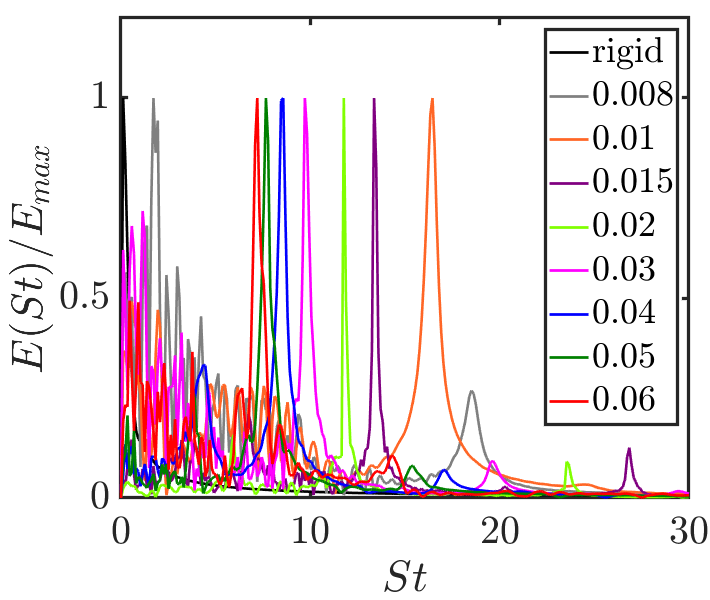
\includegraphics[width=1\linewidth]{Figures/FlowFrequency/Freq_Mode.png}
		\end{minipage} 
		\begin{minipage}[c]{0.485\linewidth}
			\begin{overpic}[width=1\linewidth]{Figures/FlowFrequency/Freq_Ca.png}
				\put(-215,200){{\parbox{1\linewidth}{$(a)$}}}	
				\put(-4,200){{\parbox{1\linewidth}{$(b)$}}}	
				\put(46,88){{\parbox{1\linewidth}{\rotatebox{87}{$transiton$}}}}
			\end{overpic}
		\end{minipage} 
		\caption{(a) Frequency energy spectra of streamwise velocity probed at slit exit next to the plate (2.2h,0.5h) is shown. The energy axis is normalized by its self maximum value. (b) Dominant frequency for the different flexible plate case, $Ca$. The cross mark in the inset figure marks the position (2.2h,0.5h).}
		\label{fig:flow_fft_S_3D}
	\end{figure}
	
	To further investigate the effect of plates' flexibility we compare the cases with different $Ca$ in figure \ref{fig:Vort_Ca}. Vorticity contours at a time instant $t/\tau=22$ are shown for rigid plate case (topmost panel) to most flexible plate case in our simulations (bottom-most panel). A qualitative overview instantly compares the effect of flexible plates with that of rigid plate case. The LVP appears to dissociate earlier for flexible plate cases additional roll-ups as second and third vortex pairs generate in sequence. However, it is worthy to note that the position of the LVPs in different case can be observed to be different positions at the same time instant indicating an effect on its propagation speed. In the figure, LVP in the case $Ca=0.04$ appears to win the race where as LVP in even more flexible plate case $(Ca=0.06)$ lags behind. Another interesting feature worth to notice is the backflow into the channel upstream. The $Ca=0.04 \ and \ 0.06$ case show a chunk of vortex structure flowing towards the inlet which shall affect the inlet flow profile.
	
	Figure \ref{fig:velpro_mean} show time-averaged velocity profiles at different sections and mean streamwise velocity for $(a)$ rigid plate case, $(b)$ $Ca=0.02$, and $(c)$ $Ca=0.06$ cases. The parabolic inlet velocity profile for rigid plate case undergo sharp rise in magnitude as it passes through the narrow slit with gap-width $\delta_g$ due to area constriction and mass flow conservation. Also, the mean flow contour show a long jet trail which indicate the absence of pinch off phenomenon in the rigid plate cases. Whereas the flexible plate reconfigure as per the inlet flow and cause larger slit gap-width $\delta_g$ (see figure \ref{fig:del_g_vs_Ca_steady}(c)) because of which the velocity profile near the slit with proportionally smaller magnitude in panel $(b)$ $Ca=0.02$ and $(c)$ $Ca=0.06$ velocity profiles. Correspondingly, the mean flow contour also reflect the similar trend and shorter jet trail is observed which suggests early dissociation of the LVP as discussed previously. The panel $c$ also confirms the interesting phenomena of backflow into the upstream and inlet velocity profile can be seen as distorted. Finally, the panel $(d)$ in the same figure shows the time-averaged Reynolds number at the centreline $Re_c$ normalized over the inlet Reynolds number $Re_\infty$ for different cases as comparison. The plot also shows trace of longer jet length for rigid plate case whereas the $Re_c$ curves for higher $Ca$ values drop closer to the slit.
	
	\subsection{Vortex pair propagation}\label{sec:vortex}
	During the periodic jetting phenomenon, the most prominent vortex structure i.e. leading vortex structure (LVP) detaches and propagates through the channel. The detached LVP speeds up through the channel. The propagation rate for different cases of $Ca$ is shown in figure \ref{fig:vortPnC}(a). The black curve represents the downstream channel propagation of the leading vortex pair for the rigid plate case. With increase in the plates' flexibility, the vortex gains a sudden release of energy as the vortex sheds off the tip of the oscillating plate. This throw increases the rate of propagation higher than that in the rigid plate case. With increasing $Ca$, the starting velocity of the leading vortex pair is shown in the \ref{fig:vortPnC}(b). Interestingly, the resulting trend is non-monotonic for the given range of $Ca$. The LVP attains highest starting velocity at the case with $Ca=0.03$ and reduces thereafter for more flexible cases. This is because cases with even more flexibility begin to cause more agitation into the flow such as back flow and interactions among the vortex pairs themselves. 
	
	\subsection{Explanation for the pinch-off of the LVP}
	 
	In the figure \ref{fig:vort_evo_1S_4S}, we show one to one comparison of the development of vortical structures in the flow over time for rigid and flexible plate ($Ca=0.02$) case. In the top panel $(a-d)$, we sequentially see the vortices shearing off the tip of each rigid plate. The vortices are shown in red as anti-clockwise flow movements and blue as clockwise. These bloom up over time and are continuously being fed to grow larger in self similar fashion. Whereas, the bottom panels $(e-f)$ in the figure are for a flexible plate case ($Ca=0.02$). The flexible plates under the effect of inlet flow inertia bends with the stream and the flow shears over the flexible plate from the fixed end to the free end. This sudden bend causes a throwback of the flow off the plates' tip in the upstream direction (panel $(e)$) in the form of vortical structures as long as the plate moves in the downstream direction. These back vortices grow gradually for a short duration but subsequently get suppressed due to the flow inertia. Now, as the flexible plate attains backward motion in the oscillation, the tip edges generate vortex in the downstream direction (panel $(f)$). This generated vortex grow as long as the next oscillation cycle of the plates kick-in which causes the change of direction in plates' motion. This sudden reversed motion cuts-off the vorticity being fed into the vortex pair and thus dissociates off the plates' edges (panel $(g)$). This vortex pair gathers vorticity and propels further into the downstream due to its self-propagating nature. This phenomena is called as "pinch-off" of the vortex pair which is found absent in the rigid plate case. It can be understood that a new time-scale in terms of flexible plate oscillations is involved in the phenomena unlike the convective time-scale as in the rigid plate case. Panel $(h)$ shows the generation of subsequent vortex pair as the next oscillation cycles prevail.
	
	\begin{figure}
		\centering
		\begin{minipage}[c]{0.48\linewidth}
			\centering
			\begin{overpic}[width=1\linewidth]{Figures/timespace/time-space_S2p1.png} 			\put(-5,165){{\parbox{1\linewidth}{$(a)$}}}	
				\put(130,35){{\parbox{1\linewidth}{$Ca=0.001$}}}	
			\end{overpic}
		\end{minipage}
			\begin{minipage}[c]{0.48\linewidth}
		\centering
		\begin{overpic}[width=1\linewidth]{Figures/timespace/time-space_S3p1.png} 				\put(-5,165){{\parbox{1\linewidth}{$(b)$}}}	
			\put(135,35){{\parbox{1\linewidth}{$Ca=0.01$}}}	
		\end{overpic}
	\end{minipage}
		\begin{minipage}[c]{0.48\linewidth}
	\centering
	\begin{overpic}[width=1\linewidth]{Figures/timespace/time-space_S4.png} 				\put(-5,165){{\parbox{1\linewidth}{$(c)$}}}	
		\put(135,35){{\parbox{1\linewidth}{$Ca=0.02$}}}	
	\end{overpic}
\end{minipage}
		\begin{minipage}[c]{0.48\linewidth}
	\centering
	\begin{overpic}[width=1\linewidth]{Figures/timespace/time-space_S5.png} 				\put(-5,165){{\parbox{1\linewidth}{$(d)$}}}	
		\put(135,35){{\parbox{1\linewidth}{$Ca=0.04$}}}	
	\end{overpic}
\end{minipage}
		\caption{(a) Normalized circulation of the leading vortex pair (LVP) over time. (b) Circulation within the LVP for flexible plate case in comparison to the rigid plate case.}
		\label{fig:time_space_all}
	\end{figure}

	It is evident from the study that steady inlet flow can be triggered to generate periodic train of vortex pair by the use of flexible plates. To analyse the shedding frequency of the these vortex pairs off the plates oscillating motion, we investigate the stream-wise velocity at a point immediately next to the slit opening ($(2.2h,0.5h)$ as a probe (see the cross mark in the inset figure of Fig~\ref{fig:flow_fft_S_3D}(b)). %The flexible plates induce more oscillations and fluctuations in the fluid system; thus, transverse velocities increase at the cost of stream-wise inertia.
	Figure \ref{fig:flow_fft_S_3D}(a), show an FFT analysis for the time signal of the probed streamwise velocity. The plot shows normalised energy spectra for the involved non-dimensional frequencies ($St_f=fh/u_{o}$, where $f$ is the streamwise flow frequency) in the time signal. In panel $b$, the dominant frequency is shown for the range of $Ca$ cases studied. We see a critical value of $St \approx 16$ at $Ca=0.01$ which marks transition from steady jet flow to pulsed oscillation of the flow in the form of periodic vortex pairs. This jump resembles similar to the classical supercritical Hopf bifurcation. Such a transformation suggests a neat periodic pumping of the steady flow. In our cases, the flexible plates act like periodic catapults which store and release energy to induce periodicity in the flow. However, thereupon at higher $Ca$ cases the corresponding flow frequency at the slit opening tends to reduce.
	
	To have an overview on the flow breakup pattern over time in the form of vortical ejections through the slit we show time-space distribution of the vertically integrated vorticity in figure \ref{fig:time_space_all}. Four different cases with $(a)\ Ca=0.001$, $(b)\ Ca=0.01$, $(c)\ Ca=0.02$, and $(d)\ Ca=0.04$ are shown in the figure. As discussed previously, the fringe pattern shows the presence of multiple vortex structures in the flow. For $Ca=0.001$, the LVP stays connected for a while before it gets unstable and further roll ups of the incoming vortices can be seen as the fringes in time-space map. In case of more flexible plate case, $Ca=0.01$ the subsequent vortices generate at early times in periodic fashion as the pinch-off phenomena is observed in the flow. Similarily, transition of steady inlet flow through the slits to periodic outflow into the downstream can be observed in even higher $Ca$ cases. In figure \ref{fig:time_space_all}(d), it is worth to notice a gap between initial trace and rest of the fringed pattern. This attributes to the higher velocity attained by the leading vortex pair in $Ca=0.04$ case because of which it leads ahead than rest of the periodic flow.
	
	\section{Summary and Conclusion}
	We have performed numerical simulations of a channel flow which passes through the wall mounted flexible plates. The small gap between the two plates act as area constriction and which results in jet like flow through it. When the plates are flexible, we see breakup of this jet due to the oscillating plates and time varying gap-width. So, the use of flexible plates in a channel flow can turn a steady flow to pulsed jet flow. We investigated this phenomenon for the plates with different flexibility (or $Ca$). An FFT analysis on the flow next the slit gap past the flexible plates reveal the flow pulsation frequency. We found a transition (or bifurcation) in the frequency analysis for $Ca>0.01$ whch also marks for the maximum flow frequency generated out of the steady input flow. We also discussed the nature and behaviour of the vortex pairs ejecting due to the periodic flow. The leading vortex pair at the start of the flow ejects faster as the $Ca=0.03$ and reaches maxima and starts to reduce on further flexibility cases. However, at higher $Ca$ cases, no distinct leading vortex pair is observed due to the chaotic advection. Finally, we present the circulation present in these leading vortex pairs.
	
	We show a method to generate periodic vortex pairs even with a steady incoming flow by the use of flexible plates. The idea of time-varying orifice diameter is realized by using plates' fluttering phenomenon. The detachment of vortex pairs without external actuation is novel and additional improvements to previous literatures. Hence, this observed phenomenon can be used in momentum transport application and also be further worked upon to fine tune and modulate the size and frequency of such periodic vortex pairs.
	
	\section*{Ackowledgments}
	We thank the fellow members of Computational Mechanics Group, IIT Kharagpur, for their support. We acknowledge research grants from the Board of Research and Nuclear Science(BRNS) and the Mathematical Research Impact Centric Support (MATRICS) scheme sponsored by the Government of India to study multiphase flow. We sincerely thank Param Shakti for computing resources developed under National Supercomputing Mission at IIT Kharagpur, India.

\bibliographystyle{elsarticle-harv} 
\bibliography{pre2}

%% else use the following coding to input the bibitems directly in the
%% TeX file.

% \begin{thebibliography}{00}

% %% \bibitem[Author(year)]{label}
% %% Text of bibliographic item

% \bibitem[ ()]{}

% \end{thebibliography}
\end{document}

\endinput
%%
%% End of file `elsarticle-template-harv.tex'.
